%
%  untitled
%
%  Created by Dean Freestone on 2010-07-06.
%  Copyright (c) 2010 . All rights reserved.
%
\documentclass[]{article}

% Use utf-8 encoding for foreign characters
\usepackage[utf8]{inputenc}

% Setup for fullpage use
\usepackage{fullpage}

% Uncomment some of the following if you use the features
%
% Running Headers and footers
%\usepackage{fancyhdr}

% Multipart figures
%\usepackage{subfigure}

% More symbols

%\usepackage{latexsym}

% Surround parts of graphics with box
\usepackage{boxedminipage}

% Package for including code in the document
\usepackage{listings}

% If you want to generate a toc for each chapter (use with book)
\usepackage{minitoc}

% This is now the recommended way for checking for PDFLaTeX:
\usepackage{ifpdf}

\usepackage{amsmath,amssymb,amsfonts} % Typical maths resource packages

\newif\ifpdf
\ifx\pdfoutput\undefined
\pdffalse % we are not running PDFLaTeX
\else
\pdfoutput=1 % we are running PDFLaTeX
\pdftrue
\fi

\ifpdf
\usepackage[pdftex]{graphicx}
\else
\usepackage{graphicx}
\fi
\usepackage[font=footnotesize]{subfig}
\usepackage{color}
\newcommand{\dean}[1]{\textsf{\emph{\textbf{\textcolor{red}{#1}}}}} 
\newcommand{\parham}[1]{\textsf{\emph{\textbf{\textcolor{blue}{#1}}}}} 

%\newcommand{\red}{\textcolor{red}}
%\newcommand{\blue}{\textcolor{blue}}
\newcommand{\cyan}{\textcolor{cyan}}

\title{Estimation of Stochastic Wilson and Cowan Neural Field Model using Expectation Maximisation Algorithm}
\author{In no specific order: Parham Aram, Dean R. Freestone, Kenneth Scerri, Michael Dewar,\\
 Andrew Zammit Mangion, David B. Grayden and Visakan Kadirkamanathan  }

\date{2010-07-06}

\begin{document}

\ifpdf
\DeclareGraphicsExtensions{.pdf, .jpg, .tif}
\else
\DeclareGraphicsExtensions{.eps, .jpg}
\fi

\maketitle


\begin{abstract}
	
	\begin{itemize}
		\item Background
		\item Method
		\item Result
		\item Conclusion
	\end{itemize}
\end{abstract}

\section{Introduction}
\begin{itemize}
	\item Understanding of macroscopic neurodynamics
	\item Neural field model
	\item Improvements in electrode technology with great spatiotemporal resolution


\end{itemize}
The aim of this paper is to create a patient-specific neural field model, by estimating parameters of a general mathematical model using data acquired from an epilepsy surgical candidate in a clinical setting. 

Instead of extracting features we aim to extract meaningful parameters...


Another recent approach for large scale neural networks based on graph theory \cite{Albert2002,Bang-Jensen2010}, employs a realistic anatomical connectivity from CoCoMac data base \cite{Kotter2004} to model resting state activity in the brain \cite{Ghosh2008,Deco2009} where each node in the network is modelled by physiologically reasonable neural population model of their internal dynamics. They perform a stability analysis of the network in terms of total connectivity and time delayes in the presence of noise. Such approach has a potential to model a virtual brain which can incorporate data from individual patient, giving insights into how patient specific features can affect its large scale neural dynamics \cite{Jirsa2010,Deco2010}.

\section{Method}

\subsection{Neural Field Model}
The neural field equations used as the parametric form of the model are based on the influential papers from Wilson and Cowan~\cite{Wilson1973}, and Amari~\cite{Amari1977}. This class of model describes a continuous cortical sheet or surface, relating mean firing rates of pre and post-synaptic neural populations. The neural field, $v\left( {\mathbf{r},t} \right)$, at position $\mathbf{r}$ and time $t$, is the aggregated post-synaptic potentials described by the \dean{(temporal convolution - I'd rather say integral equation	)} integral equation 
\begin{equation}
	\label{SpikesToPotential} v\left( {\mathbf{r},t} \right) = e^{-\zeta t}v\left( {\mathbf{r},0} \right) + \int_{0}^t {h\left( {t - t'} \right)g\left( {\mathbf{r},t'} \right)\textrm{d}t'}, 
\end{equation}   
where $v\left( {\mathbf{r},0} \right)$ is the membrane voltage at the initial time $t = 0$, $h(\cdot)$ is the synaptic response kernel assumed to be first order and of the form 
\begin{equation}
	\label{SynapticRespKernel} h(t) = \eta(t)\exp{\left(-\zeta t\right)}, 
\end{equation}
\cyan{small thing: are we using $\exp(x)$ or $e^x$ to represent exponential?}
$\zeta=\tau^{-1}$, $\tau$ is the synaptic time constant and $\eta(t)$ is the Heaviside step function \parham{(you can keep it here if you wish as it doesn't change the integral equation because of the upper limit. I would remove it)}. $g(\cdot)$ describes the mean firing rate. In practice, the firing rate can rarely be considered as a purely determinstic process because \dean{(can someone write down why?)}. We thus choose to introduce a spatially coloured space-time Wiener process $W(\mathbf{r},t)$ to model the flactuations in the mean firing rate and decompose $g(\cdot)$ as
\begin{equation}\label{DecompositionOfg}
g(\mathbf{r},t)\textrm{d}t = \tilde{g}(\mathbf{r},t)\textrm{d}t + \sigma_W \textrm{d}W(\mathbf{r},t) 
\end{equation}
where $\sigma_W \ge 0$ is a measure of the introduced space-time randomness. For $\sigma_W = 0$ a pure deterministic process is recovered. As a result of the random component, for $\sigma_W > 0$, the membrane voltage $v(\mathbf{r},t)$ is itself a stochastic process. Assuming an infinite propagation velocity for action potentials within the field, the deterministic incoming firing rate is described by a spatial convolution \dean{citation?}
\begin{equation}
	\label{RateBasedInteractions} \tilde{g}\left( \mathbf{r},t \right) = \int_\Omega {w\left( \mathbf{r},\mathbf{r}' \right)f\left( v\left( \mathbf{r}',t \right) \right)\textrm{d}\mathbf{r}'}, 
\end{equation}
where $w(\cdot)$ is the spatial connectivity kernel and $\Omega$ is the spatial domain representing the cortical sheet or surface. The function $f(\cdot)$ relates mean post-synaptic potentials to mean firing rates and follows a sigmoid described by
\begin{equation}
	\label{ActivationFunction} f\left( v\left( \mathbf{r}', t \right) \right) = \frac{1}{1 + \exp \left( \varsigma \left( v_0 - v\left(\mathbf{r}',t\right) \right) \right)}, 
\end{equation}
where $v_0$ and $\varsigma$ describe the firing threshold and the slope of the sigmoid respectively. 
By substituting equation~\ref{DecompositionOfg} into equation~\ref{SpikesToPotential} we obtain the stochastic integral equation model 
\begin{equation}
	\label{StochasticModel} v\left(\mathbf{r},t\right) = e^{-\zeta t}v\left( {\mathbf{r},0} \right) +
	\int_{0}^t h\left(t - t'\right)\tilde{g}\left(\mathbf{r},t'\right) \textrm{d}t'+ \sigma_W\int_{0}^t h\left(t - t'\right)\textrm{d}W\left(\mathbf{r},t'\right).
\end{equation}
 Here we assume that $v\left( {\mathbf{r}},0 \right)$ is independent of the disturbance on the action potentials and assumed to be generated by a known distribution. We stress that $\sigma_W$ does not depend on the field $v({\mathbf{r}},t)$ and hence the noise in equation \ref{StochasticModel} is strictly additive. The general integral-differential equation is given by 
\begin{equation} \label{DifferentialEquationContTime}
 \textrm{d}v(\mathbf{r},t) + \zeta v(\mathbf{r},t)\textrm{d}t = \tilde{g}(\mathbf{r},t)\textrm{d}t + \textrm{d}W(\mathbf{r},t)  ~~~~ t \ge 0, v(\mathbf{r},0) = \cyan{GP?}
\end{equation}
To show that this is indeed the case consider the function $\kappa(v(\mathbf{r},t),t) = v(\mathbf{r},t)e^{\zeta t}$. We note that $\kappa(v(\mathbf{r},t),t)$ is twice differentiable so that we can apply Ito's formula to obtain
\begin{equation}
 \textrm{d}\kappa = e^{\zeta t}g(\mathbf{r},t)\textrm{d}t + e^{\zeta t}\sigma \textrm{d}W(\mathbf{r},t)
\end{equation}
\noindent Integrating over $[0,t]$ and multiplying throughout by $e^{-\zeta t}$ gives the required result.
The neural field equations must be written as a discrete-time finite-dimensional model in order to relate it to patient-specific data. The discrete-time model is found applying the a first-order Euler-Maruyama method on equation \ref{DifferentialEquationContTime} giving
\begin{equation}\label{EulerMethod}
	v\left( \mathbf{r},t+T_s \right)-v\left( \mathbf{r},t \right) + \zeta T_sv\left(\mathbf{r},t \right) = T_s\int_\Omega {w\left( \mathbf{r},\mathbf{r}' \right) f\left( {v\left( \mathbf{r}',t \right)}\right)\textrm{d}\mathbf{r}'} + 	\sigma_W[W\left( \mathbf{r},t+T_s \right)-W\left( \mathbf{r},t \right)],
\end{equation}
where $T_s$ is the time step or sampling period. To simplify the notation, the sample at the the current time step shall be indexed by $t$ and the future time step by $t+1$ for the rest of the paper. Rearranging equation~\ref{EulerMethod} gives the integro-difference equation (IDE) form
\begin{equation}
	\label{NoisyDiscreteTimeModel} 
	v_{t+1}\left(\mathbf{r}\right) = 
	\xi v_t\left(\mathbf{r}\right) + 
	T_s \int_\Omega { 
	    w\left(\mathbf{r},\mathbf{r}'\right)
	    f\left(v_t\left(\mathbf{r}'\right)\right) 
	\textrm{d}\mathbf{r}'} 
	+ e_t\left(\mathbf{r}\right), 
\end{equation}
where $e_t(\mathbf{r}) = \sigma_W[W\left( \mathbf{r},t+T_s \right)-W\left( \mathbf{r},t \right)]$ is the increment of a space-time Wiener process, $i.i.d.$ with zero spatial mean such that $e_t(\mathbf{r})\sim\mathcal{GP}(\mathbf 0,\sigma_d^2\gamma(\mathbf{r}-\mathbf{r}'))$, where $\sigma_d^2=T_s\sigma_W^2$. Here $\mathcal{GP}(\mathbf 0,\sigma_d^2\gamma(\mathbf{r}-\mathbf{r}'))$ denotes a zero mean spatial Gaussian process with covariance function $\gamma(\mathbf{r}-\mathbf{r}')$~\cite{Rasmussen2005}.
To reduce the model to a finite-dimensional system the neural field is approximated by a basis function decomposition where
\begin{equation}
	\label{DefFieldDecomp} v_t\left(\mathbf{r}\right) \approx \boldsymbol{\phi}^{\top}\left(\mathbf{r}\right) \mathbf{x}_t 
\end{equation}
and $\mathbf{x}_t$ is a state vector that weights a vector of two-dimension Gaussian basis functions, $\boldsymbol{\phi}(\mathbf{r})$, described by
\begin{equation}\label{eq:FieldBasisFunction}
	\boldsymbol\phi\left(\mathbf{r}-\mathbf{r}'\right) =
\exp{\left(-\frac{(\mathbf{r}-\mathbf{r}')^\top(\mathbf{r}-\mathbf{r}')}{\sigma_{\phi}^2}\right)}. 
\end{equation}
The parameter $\sigma_{\phi}$ controls the basis function width and is inferred by frequency analysis. Substituting equation~\ref{DefFieldDecomp} into~\ref{NoisyDiscreteTimeModel} gives to approximate model
\begin{equation}
	\label{eq:reduced continuous model}
	\boldsymbol{\phi}^{\top}(\mathbf{r})\mathbf{x}_{t+1}= T_s\int_\Omega{f(\boldsymbol{\phi}^{\top}(\mathbf{r}')\mathbf{x}_t )w(\mathbf{r},\mathbf{r}')\textrm{d}\mathbf{r}'}
	+ \xi\boldsymbol{\phi}^{\top}(\mathbf{r})x_t + e_t(\mathbf{r}). 
\end{equation}
Next we multiply equation~\ref{eq:reduced continuous model} by $\boldsymbol{\phi}(\mathbf{r})$ and integrate over the spatial domain, $\Omega$, to get 
\begin{equation}
	\label{StartofReduction}
 	\int_\Omega {\boldsymbol{\phi} \left(\mathbf{r}\right)\boldsymbol{\phi}^{\top}\left(\mathbf{r}\right) \textrm{d}\mathbf{r}} \mathbf{x}_{t+1} = T_s \int_\Omega {\boldsymbol{\phi} (\mathbf{r}) \int_\Omega {w(\mathbf{r},\mathbf{r}') f(\boldsymbol{\phi}^{\top}(\mathbf{r}') \mathbf{x}_t ) \textrm{d}\mathbf{r}'}\textrm{d}\mathbf{r}} + \xi\int_\Omega{\boldsymbol{\phi}(\mathbf{r})\boldsymbol{\phi}^{\top}(\mathbf{r})\textrm{d}\mathbf{r}} \mathbf{x}_t + \int_\Omega{\boldsymbol{\phi} (\mathbf{r}) e_t(\mathbf{r})\textrm{d}\mathbf{r}}. 
\end{equation}
Now by defining the matrix
\begin{equation}\label{eq:DefGamma}
	\boldsymbol{\Gamma} \triangleq \int_\Omega {\boldsymbol{\phi} \left(\mathbf{r}\right)\boldsymbol{\phi} ^{\top}\left(\mathbf{r}\right)\textrm{d}\mathbf{r}} 
\end{equation}
enables the pseudo inverse of $\boldsymbol{\phi(\mathbf{r})}$ to be taken, such that the state vector is isolated on the left-hand-side as
\begin{equation}\label{eq:ReducedForm}
	 \mathbf{x}_{t+1} = T_s\boldsymbol{\Gamma}^{-1}
	 \int_\Omega \boldsymbol{\phi}(\mathbf{r}) 
	 \int_\Omega w(\mathbf{r},\mathbf{r}')f(\boldsymbol{\phi}^{\top}(\mathbf{r}')\mathbf{x}_t) \textrm{d}\mathbf{r}' \textrm{d}\mathbf{r} 
	 + \xi\mathbf{x}_t + \boldsymbol{\Gamma}^{-1} \int_\Omega{\boldsymbol{\phi}(\mathbf{r}) e_t(\mathbf{r})\textrm{d}\mathbf{r}}.
\end{equation}
A property of the basis function decomposition it the preservation of the Gaussianality of the disturbance term. The decomposition disturbance term is defined as
\begin{equation}\label{eq:Wt} 
	\mathbf{e}_t \triangleq \boldsymbol{\Gamma}^{-1}\int_\Omega {\boldsymbol{\phi} ( \mathbf{r} )e_t( \mathbf{r} )\textrm{d}\mathbf{r}},
\end{equation}
where $\mathbf{e}_t \sim\mathcal{N}(\mathbf 0,\boldsymbol\Sigma_e)$. The covariance matrix is defined as (see the Supporting Information, S1, for the derivation)
\begin{equation}
	\boldsymbol\Sigma_e \triangleq \sigma_d^2\mathbf{\Gamma}^{-1}\int_{\Omega}\int_{\Omega}\boldsymbol{\phi}\left(\mathbf r\right) \gamma\left(\mathbf r- \mathbf r' \right)\boldsymbol{\phi}\left(\mathbf r'\right)^{\top}d\mathbf r' d\mathbf r\mathbf{\Gamma}^{- \top}. 
\end{equation}

To relate the model to the data the electrodes are also modelled. The electrodes have a pick-up range (for LFPs) of approximately 400~$\mu$m. Therefore, we model the electrodes as a spatial convolution of a Gaussian shaped sensor kernel (using a width parameters of 400~$\mu$m) with the neural field. The observation equation is
\begin{equation}
    \label{eq:ObservationEquation}
	\mathbf{y}_t =
	\int_{\Omega}{
	    m\left(\mathbf{r}_n-\mathbf{r}'\right)v_t\left(\mathbf{r}'\right)
	\textrm{d}\mathbf{r}'} + 
	\boldsymbol{\varepsilon}_t, 
\end{equation}
where $\mathbf{r}_n$ defines the location of the sensors in the field, $n=1,...,N$ indexes the sensors and $\boldsymbol{\varepsilon}_t \sim \mathcal{N}\left(0,\boldsymbol{\Sigma}_{\varepsilon}\right)$. $\mathcal{N}\left(0,\boldsymbol{\Sigma}_{\varepsilon}\right)$ denotes the multivariate normal distribution with mean zero and covariance matrix $\boldsymbol{\Sigma}_{\varepsilon}$. The sensor kernel, $m(\mathbf{r}-\mathbf{r}')$, is defined by 
\begin{equation}
	m\left(\mathbf{r}-\mathbf{r}'\right) = \exp{\left(-\frac{(\mathbf{r}-\mathbf{r}')^\top(\mathbf{r}-\mathbf{r}')}{\sigma_m^2}\right)},
\end{equation}
where $\sigma_m$ sets the sensor width. Under the assumption that the basis function decomposition is accurate, the observation equation of the reduced model is found by substituting equation~\ref{DefFieldDecomp} into~\ref{eq:ObservationEquation} giving
\begin{equation}\label{eq:ReducedObservationEquation}
	\mathbf{y}_t = \int_{\Omega}{m\left(\mathbf{r}_n-\mathbf{r}'\right)\boldsymbol{\phi}^{\top}\left(\mathbf{r'}\right) \mathbf{x}_t\textrm{d}\mathbf{r}'} + \boldsymbol{\varepsilon}_t. 
\end{equation}
The observation equation is linear with respect to the state and can be written in the more compact form
\begin{equation}\label{ObservationEquation} 
	\mathbf{y}_t = \mathbf{C}\mathbf{x}_t + \boldsymbol{\varepsilon}_t,
\end{equation}
where the observation matrix is 
\begin{equation}
	\mathbf{C} = \left[
	\begin{array}{{ccc}} 
		c_{1,1} & \dots & c_{1,L} \\
		\vdots & \ddots & \vdots \\
		c_{N,1} & \dots & c_{N,L} 
	\end{array}
	\right] 
\end{equation}
and 
\begin{equation}
	c_{i,j} = \int_{\Omega}m(\mathbf{r}_i - \mathbf{r}')\boldsymbol{\phi}_j(\mathbf{r}')\textrm{d}\mathbf{r}'. 
\end{equation}

\dean{I will do the connectivity kernel decomposition bit after the correlation analysis, because we can use it to say something about heterogeneity and isotropy.}

\subsection{Correlation analysis}\label{subsec:CorrAnal}
Under the assumption that the sensors are not spatially band-limiting the spectral content of the field and the connectivity kernel is homogeneous, the support for the connectivity kernel can be inferred by studying the spatial cross-correlation between consecutive observations. The deterministic component of the spatial mapping between consecutive fields is due to the convolution of the connectivity kernel with the firing rates. Although the relationship between the field and the firing rate is nonlinear, the cross-correlation analysis still extracts meaningful results. This can be seen by considering the three operating regions of the sigmoid. When the mean membrane voltage is below the active region of the sigmoid, the firing rate will be approximately zero and only very small spatial correlations will observed. Therefore, this will not contribute to the results. Within the active region the sigmoid can be approximated by a linear function between consecutive samples, given a sufficiently high sampling rate. Therefore, linear cross-correlation analysis is appropriate. When the sigmoid is in the saturated region, the correlation coefficients will be higher, but not provide a meaningful measure of the kernel weight or gain. Therefore, we can not estimate the gain for the kernel using cross-correlation analysis, but the spatial extent can still be inferred. The gain for the kernel will be inferred using the EM algorithm described below.

\subsubsection{Estimation of Connectivity Kernel Support}
For the derivation of the spatial properties estimator of the neural field equations a more compact notation is employed to define convolution and correlation operators. The spatial convolution shall be denoted as
\begin{equation}
	\int_\Omega a(\mathbf{r}-\mathbf{r}')b(\mathbf{r}')d\mathbf{r}' = (a\ast b)(\mathbf{r}),
\end{equation}
and the spatial cross-correlation shall be denoted as 
\begin{equation}
	\int_\Omega a(\mathbf{r})b(\mathbf{r}+\boldsymbol{\iota})d\mathbf{r} = (a\star b)(\boldsymbol{\iota}),
\end{equation} 
where $\iota$ is the spatial shift. The spatial relationship between consecutive observations is governed by the shape of the connectivity kernel. Therefore, the spatial cross-correlation between consecutive observations is used to estimate the kernel's support and shape. To begin the derivation the spatial cross-correlation between consecutive observations (in time) is defined as
\begin{equation}
	R_{y_{t+1}y_t}(\boldsymbol{\iota}) = \left(y_{t+1}\star y_t\right)\left(\boldsymbol{\iota}\right),
\end{equation}
 The aim of the derivation is to make the necessary substitutions and simplifications to get an expression of the cross-correlation as a function of the connectivity kernel. In the next step equation~\eqref{eq:EM-ObservationEquation} is substituted for $y_{t+1}(\mathbf{r})$ and expanded to give
\begin{equation}
	R_{y_{t+1}y_t}\left(\boldsymbol{\iota}\right) = \left(\left(m \ast v_{t+1}\right)\star y_t\right)\left(\boldsymbol{\iota}\right) + \left(\varepsilon_{t+1} \star y_t\right)\left(\boldsymbol{\iota}\right).
\end{equation}
Next equation~\eqref{eq:EM-DiscreteTimeModel} is substituted for $v_{t+1}(\mathbf{r})$ giving 
\begin{align}
	R_{y_{t+1}y_t}(\boldsymbol{\iota}) &= (\left(m \ast \left(\xi v_t +  T_s g_t + e_t\right)\right) \star y_t)(\boldsymbol{\iota})\\
	&= \xi\left(\left(m \ast v_t\right) \star y_t \right)(\boldsymbol{\iota}) \nonumber\\
	&\quad+ T_s \left(\left(m\ast g_t\right)\star y_t \right)(\boldsymbol{\iota}) \nonumber\\
	&\quad+ \left(\left(m\ast e_t\right)\star y_t \right)(\boldsymbol{\iota}) \nonumber\\
	&\quad+ (\varepsilon_{t+1} \star y_t)(\boldsymbol{\iota}).
\end{align}
Now the expectation over time is taken, so that the observation noise and process disturbance terms have minimal effect on the result, giving 
\begin{align}\label{eq:EM-ExpectationToCancelNoise}
	\mathbf{E}[R_{y_{t+1}y_t}(\boldsymbol{\iota})] &= \mathbf{E}[\xi\left(\left(m \ast v_t\right) \star y_t \right)(\boldsymbol{\iota})] + T_s \mathbf{E}[\left(\left(m\ast g_t\right)\star y_t \right)(\boldsymbol{\iota})],
\end{align}
since the disturbance and measurement noise are assumed to be independent of the observations and temporally white. 
The cross-correlation is further simplified by recognizing that the first term on right hand side of equation~\eqref{eq:EM-ExpectationToCancelNoise} can be written as 
\begin{align}
	\mathbf{E}[\xi&\left(\left(m \ast v_t \right) \star y_t \right)(\boldsymbol{\iota})] = \mathbf{E}\left[\xi\left(\left(y_t-\varepsilon_t\right) \star y_t \right)(\boldsymbol{\iota})\right] \nonumber \\
	&= \xi \mathbf{E}\left[ (y_t \star y_t)(\boldsymbol{\iota}) - \left(\varepsilon_t\star y_t \right)(\boldsymbol{\iota})\right] \nonumber \\
	&= \xi\mathbf{E}[ R_{y_ty_t}(\boldsymbol{\iota})  - \left(\varepsilon_t \star (m\ast v_t + \varepsilon_t)\right) (\boldsymbol{\iota})] \nonumber \\
	&=\xi\mathbf{E}[ R_{y_ty_t}(\boldsymbol{\iota}) -\left(\varepsilon_t\star (m\ast v_t)\right)(\boldsymbol{\iota}) - (\varepsilon_t\star\varepsilon_t)(\boldsymbol{\iota})] \nonumber \\
	&= \xi\left(\mathbf{E}[ R_{y_ty_t}(\boldsymbol{\iota})] - \sigma_{\varepsilon}^2 \delta(\boldsymbol{\iota})\right), \label{eq:EM-FirstTermReduced}
\end{align}
where $\delta\left(\cdot\right)$ denotes Kronecker delta. Substituting equation~\eqref{eq:EM-FirstTermReduced} back into equation~\eqref{eq:EM-ExpectationToCancelNoise} gives
\begin{align}\label{eq:EM-SimplifiedFirstTerm}
	\mathbf{E}[R_{y_{t+1}y_t}(\boldsymbol{\iota})] &= \xi\left(\mathbf{E}[ R_{y_ty_t}(\boldsymbol{\iota})] - \sigma_{\varepsilon}^2 \delta(\boldsymbol{\iota})\right)+ T_s\mathbf{E}[ \left(\left(m\ast g_t\right)\star y_t \right)(\boldsymbol{\iota})].
\end{align}
Next we simplify second term in equation~\eqref{eq:EM-SimplifiedFirstTerm} to get an expression involving the connectivity kernel. By substituting equation~\eqref{eq:EM-RateBasedInteractions} for $g_t$ we can write
\begin{equation}\label{eq:EM-before_linearization}
	T_s((m \ast g_t) \star y_t)(\boldsymbol\iota) = T_s((w \ast m\ast f(v_t)) \star y_t)(\boldsymbol\iota).
\end{equation}
The remainder of the derivation is focused on isolating the connectivity kernel. To show how this is done, the activation function is assumed to be in the linear region, i.e 
 \begin{equation}
	f\left(v_t(\mathbf{r})\right) \approx \varsigma v_t(\mathbf{r})
\end{equation} 
Substituting the linear activation function back into equation~\eqref{eq:EM-before_linearization} yields
\begin{align}\label{eq:EM-after_linearization1}	
	T_s((m \ast g_t) \star y_t)(\boldsymbol\iota) &\approx T_s\varsigma((w \ast m\ast v_t) \star y_t)(\boldsymbol\iota).
\end{align}
Now by substituting $y_t - \varepsilon_t$ in for $m\ast v_t$ equation \eqref{eq:EM-after_linearization1} can be written as 
\begin{align}
	T_s((m \ast g_t) \star y_t)(\boldsymbol\iota) &\approx T_s\varsigma(w\ast (y_t - \varepsilon_t)) \star y_t (\boldsymbol\iota)
\end{align}
To isolate the kernel, the order of the convolution and cross-correlation is reversed by recognizing that a property $(a \ast b)(\boldsymbol\iota) \star c(\boldsymbol\iota) = a(-\boldsymbol\iota)\ast(b \star c)(\boldsymbol\iota)$ \parham{(see Appendix for proof)}. Therefore,
\begin{align}
	T_s((m \ast g_t) \star y_t)(\boldsymbol\iota) &\approx T_s\varsigma w(-\boldsymbol\iota) \ast ((y_t - \varepsilon_t)) \star y_t)(\boldsymbol\iota),
\end{align}
Now using the identity established to get equation~\eqref{eq:EM-FirstTermReduced} gives
\begin{equation}\label{eq:EM-second_term_reduced}
	T_s\mathbf{E}\left[((m \ast g_t) \star y_t)(\boldsymbol\iota)\right] \approx T_s\varsigma w(-\boldsymbol\iota) \ast  (\mathbf{E}\left[R_{y_ty_t}(\boldsymbol\iota)\right] - \sigma_{\varepsilon}^2 \delta(\boldsymbol\iota))
\end{equation}
Now substituting back equation~\eqref{eq:EM-second_term_reduced} into equation~\eqref{eq:EM-SimplifiedFirstTerm} gives
\begin{align}\label{eq:EM-SimplifiedXcorr}
	\mathbf{E}[R_{y_{t+1}y_t}(\boldsymbol{\iota})] &= \xi\left(\mathbf{E}[ R_{y_ty_t}(\boldsymbol{\iota})] - \sigma_{\varepsilon}^2 \delta(\boldsymbol{\iota})\right)\nonumber \\
&+T_s\varsigma w(-\boldsymbol\iota) \ast  (\mathbf{E}\left[R_{y_ty_t}(\boldsymbol\iota)\right] - \sigma_{\varepsilon}^2 \delta(\boldsymbol\iota))
\end{align}
Rearranging equation~\eqref{eq:EM-SimplifiedXcorr} gives
\begin{align}
	 w(-\boldsymbol\iota) \ast  (\mathbf{E}\left[R_{y_ty_t}(\boldsymbol\iota)\right] - \sigma_{\varepsilon}^2 \delta(\boldsymbol\iota))&=\frac{1}{T_s\varsigma}\mathbf{E}[R_{y_{t+1}y_t}(\boldsymbol{\iota})]-\frac{\xi}{T_s\varsigma}\left(\mathbf{E}[ R_{y_ty_t}(\boldsymbol{\iota})] - \sigma_{\varepsilon}^2 \delta(\boldsymbol{\iota})\right)\nonumber \\
\end{align}
The solution of the above equation for the connectivity kernel is a deconvolution. This can be approached from a number of different standpoints. The simplest solution is to use the convolution theorem and to solve for the kernel algebraically in the frequency domain.
\begin{align}\label{eq:EM-XcorrFourier}
	\mathcal{F}\{w(-\boldsymbol\iota)\} \mathcal{F}\{(\mathbf{E}\left[R_{y_ty_t}(\boldsymbol\iota)\right] - \sigma_{\varepsilon}^2 \delta(\boldsymbol\iota))\} &\approx \frac{1}{T_s\varsigma}\mathcal{F}\{\mathbf{E}[R_{y_{t+1}y_t}(\boldsymbol{\iota})]\}\nonumber \\
&-\frac{\xi}{T_s\varsigma}\mathcal{F} \{\left(\mathbf{E}[ R_{y_ty_t}(\boldsymbol{\iota})] - \sigma_{\varepsilon}^2 \delta(\boldsymbol{\iota})\right)\}.
\end{align}
Now rearranging \eqref{eq:EM-XcorrFourier} gives
\begin{equation}\label{eq:EM-Fourier_TF_of_Kernel}
	\mathcal{F}\left(w(-\boldsymbol\iota)\right) = \frac{1}{T_s\varsigma }\left[\frac{\mathcal{F}\{\mathbf{E}[R_{y_{t+1}y_t}(\boldsymbol{\iota})]\}}{\mathcal{F}\{(\mathbf{E}\left[R_{y_ty_t}(\boldsymbol\iota)\right] - \sigma_{\varepsilon}^2 \delta(\boldsymbol\iota))\}}-\xi\right].
\end{equation}
From \eqref{eq:EM-Fourier_TF_of_Kernel} it can be observed that an error in our guess for $\xi$ will result in a dilation or contraction of the estimated kernel support and an incorrect estimate in the observation noise will result in a distortion in the shape of the kernel, however if the signal to noise ratio is high such a distortion would be insignificant. The denominator in equation \eqref{eq:EM-Fourier_TF_of_Kernel} is in fact the power spectral density of noise free observations which is non-negative and real. This important result is known as Weiner-Khintchine (W-K) theorem in signal processsing which states that the power spectral density of the wide sense stationary process is the Fourier transform of its autocorrelation function \cite{Ricker2003}. The numerator is also called the cross spectrum or cross spectral density. Since the connectivity kernel is a real function, the following relation holds \cite{Bracewell2000}
\begin{equation}
 \mathcal{F}\left(w(\boldsymbol\iota)\right)=\overline{\mathcal{F}\left(w(-\boldsymbol\iota)\right)},
\end{equation}
where over-bar denotes complex conjugate operator. Finally, an expression for the kernel is obtained by taking the inverse Fourier tranform 
\begin{equation}\label{eq:KernelSolution}
	w(\boldsymbol\iota) = \frac{1}{T_s\varsigma }\mathcal{F}^{-1}\overline{\left\{\frac{\mathcal{F}\{\mathbf{E}[R_{y_{t+1}y_t}(\boldsymbol{\iota})]\}}{\mathcal{F}\{(\mathbf{E}\left[R_{y_ty_t}(\boldsymbol\iota)\right]\} - \sigma_{\varepsilon}^2 }-\xi\right\}}.
\end{equation}
Complex conjugate operator essentially reflects the connectivity kernel through the origin in the spatial domain, therefore, if the connectivity kernel is isotropic, the complex conjugate operator can be dropped. 
% Alternatively, the convolution can be written as a system of linear equations by forming the convolution (Toeplitz) matrix. The solution of the convolution equation for $w(\cdot)$ can then be found by either inverting the convolution matrix or directly solving the system of equations.  
% Directly solving the system is the most numerically stable and less computationally demanding then inverting the convolution matrix. To show this we take the spatial Fourier transform of both sides of equation~\ref{} giving
\subsubsection{Estimation of Disturbance Covariance Support}
The observation auto-correlation at time $t+1$ can be expressed as
\begin{equation}
	R_{y_{t+1}y_{t+1}}(\boldsymbol{\iota})=(y_{t+1} \star y_{t+1})(\boldsymbol\iota).
\end{equation}
Substituting equation~\eqref{eq:EM-ObservationEquation} in for $y_{t+1}$ and expanding gives
\begin{align}\label{eq:EM-expanded_auto_corr}
	R_{y_{t+1}y_{t+1}}(\boldsymbol{\iota}) &= \xi((m \ast v_{t}) \star y_{t+1})(\boldsymbol{\iota}) +T_s((m\ast g_{t})\star y_{t+1})(\boldsymbol{\iota}) \nonumber \\
	&+((m\ast e_{t})\star  y_{t+1})(\boldsymbol{\iota})+(\varepsilon_{t+1} \star y_{t+1})(\boldsymbol{\iota}).
\end{align}
By using similar arguments that were used in the derivation for the connectivity kernel support, the autocorrelation can be simplified by recognizing that
\begin{align}\label{eq:EM-Autoterm1}
  \mathbf{E}[\xi((m\ast v_{t})\star y_{t+1})(\boldsymbol{\iota})]&=\xi \mathbf{E}[ R_{y_ty_{t+1}}(\boldsymbol{\iota})],
\end{align}
and
\begin{align}\label{eq:EM-Autoterm2}
	T_s\mathbf{E}[((m\ast g_t) \star y_{t+1})(\boldsymbol\iota)] &\approx T_s\varsigma\mathbf{E}[((m \ast w )\star y_{t+1})(\boldsymbol\iota)] \nonumber\\
	&= T_s\varsigma w(-\boldsymbol\iota) \ast (\mathbf{E}\left[R_{y_ty_{t+1}}(\boldsymbol\iota)\right] ).
\end{align}
\begin{align}\label{eq:EM-Autoterm3}
 \mathbf{E}[(\varepsilon_{t+1}\star y_{t+1})(\boldsymbol\iota)]&=\sigma_{\varepsilon}^2\delta(\boldsymbol{\iota}),
\end{align}
Substituting equations~\eqref{eq:EM-Autoterm1}, \eqref{eq:EM-Autoterm2}, and ~\eqref{eq:EM-Autoterm3} back into equation~\eqref{eq:EM-expanded_auto_corr} gives
\begin{align}\label{eq:EM-Auto&CrossNoisy}
	\mathbf{E}[R_{y_{t+1}y_{t+1}}(\boldsymbol{\iota})] &= \xi \mathbf{E}[R_{y_ty_{t+1}}(\boldsymbol{\iota})]+T_s\varsigma w(-\boldsymbol\iota) \ast (\mathbf{E}\left[R_{y_ty_{t+1}}(\boldsymbol\iota)\right] ) \nonumber \\
	&+\mathbf{E}[((m\ast e_t)\star y_{t+1})(\boldsymbol\iota)] +\sigma_{\epsilon}^2\delta(\boldsymbol{\iota}).
\end{align}
The third term in \eqref{eq:EM-Auto&CrossNoisy} can be simplified as
\begin{align}\label{eq:EM-term3Noisy}
\mathbf{E}[((m\ast e_t)\star y_{t+1})(\boldsymbol\iota)] &= \mathbf{E}[((m\ast e_t)\star (m\ast v_{t+1}+\varepsilon_{t+1})) (\boldsymbol\iota)] \nonumber \\
	&= \mathbf{E}[(\left(m \ast e_t\right) \star (m \ast [\xi v_t + T_s g_t + e_t]+\varepsilon_{t+1}))(\boldsymbol\iota)] \nonumber \\
	&=\mathbf{E}[\left(m \ast e_t\right)\star\left(m \ast e_t\right)(\boldsymbol\iota)]
\end{align}
A property of cross-correlation and convolution is $(a \ast b)(\boldsymbol\tau) \star (a \ast b)(\boldsymbol\tau)=(a \star a)(\boldsymbol\tau)\ast(b \star b)(\boldsymbol\tau)$ \parham{(see Appendix II for a proof)}, using the isotropy property of the observation kernel we can write
\begin{align}\label{eq:EM-Autoterm4}
\mathbf{E}[(\left(m \ast e_t\right)\star\left(m \ast e_t\right))(\boldsymbol\iota)]&=\mathbf{E}[(\left(m \star m\right)\ast\left(e_t \star e_t\right))(\boldsymbol\iota)] \nonumber \\
&=(m\ast m \ast \gamma)(\boldsymbol\iota).
\end{align}
Substituting this back into equation~\eqref{eq:EM-Auto&CrossNoisy} gives
\begin{align}
	\mathbf{E}[R_{y_{t+1}y_{t+1}}(\boldsymbol{\iota})] &= \xi \mathbf{E}[R_{y_ty_{t+1}}(\boldsymbol{\iota})]+T_s\varsigma w(-\boldsymbol\iota) \ast (\mathbf{E}\left[R_{y_ty_{t+1}}(\boldsymbol\iota)\right] ) \nonumber \\
	&+(m\ast m \ast \gamma)(\boldsymbol\iota) +\sigma_{\epsilon}^2\delta(\boldsymbol{\iota}).
\end{align}
To solve for the disturbance covariance, again the convolution theorem is applied to perform the deconvolution algebraically. Taking the Fourier transform and rearranging gives
\begin{align}
	\mathcal{F}\{(m\ast m \ast \gamma)(\boldsymbol\iota)\} &= \mathcal{F}\{\mathbf{E}[R_{y_{t+1}y_{t+1}}(\boldsymbol{\iota})]\}-\xi \mathcal{F}\{\mathbf{E}[R_{y_ty_{t+1}}(\boldsymbol{\iota})]\}\nonumber \\ 
	&- T_s\varsigma\mathcal{F}\{w(-\boldsymbol\iota)\}\mathcal{F}\left\{\mathbf{E}\left[R_{y_ty_{t+1}}(\boldsymbol\iota)\right] \right\}-\sigma_{\varepsilon}^2 
\end{align}
Now substituting in equation~\eqref{eq:EM-Fourier_TF_of_Kernel} for $\mathcal{F}\{w(-\boldsymbol{\iota})\}$ results in
\begin{align}
	\mathcal{F}&\{(m\ast m \ast \gamma)(\boldsymbol\iota)\} = \mathcal{F}\{\mathbf{E}[R_{y_{t+1}y_{t+1}}(\boldsymbol{\iota})]\}-\xi \mathcal{F}\{\mathbf{E}[R_{y_ty_{t+1}}(\boldsymbol{\iota})]\}\nonumber \\ 
	&- T_s\varsigma \times \frac{1}{T_s\varsigma }\left[\frac{\mathcal{F}\{\mathbf{E}[R_{y_{t+1}y_t}(\boldsymbol{\iota})]\}}{\mathcal{F}\{(\mathbf{E}\left[R_{y_ty_t}(\boldsymbol\iota)\right] - \sigma_{\varepsilon}^2 \delta(\boldsymbol\iota))\}}-\xi\right]\mathcal{F}\left\{\mathbf{E}\left[R_{y_ty_{t+1}}(\boldsymbol\iota)\right] \right\} -\sigma_{\varepsilon}^2\label{eq:EM=mmgamma}
\end{align}
Now simplifying gives
\begin{align}\label{eq:EM-MMGFourier1}
	\mathcal{F}&\{m(\boldsymbol\iota)\}\mathcal{F}\{m(\boldsymbol\iota)\}\mathcal{F}\{\gamma(\boldsymbol\iota)\} = \nonumber \\
&\mathcal{F}\{\mathbf{E}[R_{y_{t+1}y_{t+1}}(\boldsymbol{\iota})]\}- \left[\frac{\mathcal{F}\{\mathbf{E}[R_{y_{t+1}y_t}(\boldsymbol{\iota})]\}\mathcal{F}\left\{\mathbf{E}\left[R_{y_ty_{t+1}}(\boldsymbol\iota)\right] \right\}}{\mathcal{F}\{(\mathbf{E}\left[R_{y_ty_t}(\boldsymbol\iota)\right]\} - \sigma_{\varepsilon}^2}\right]-\sigma_{\varepsilon}^2 ,
\end{align}
rearranging and taking inverse Fourier transform gives the final result
\begin{align}\label{eq:EM-MMGFourier2}
	&\gamma(\boldsymbol\iota) = \nonumber \\
&\mathcal{F}^{-1}\left\lbrace \frac{1}{\tilde{m}(\boldsymbol\iota)}\left[\left[\mathcal{F}\{\mathbf{E}[R_{y_{t+1}y_{t+1}}(\boldsymbol{\iota})]\}-\sigma_{\varepsilon}^2\right]- \left[\frac{\mathcal{F}\{\mathbf{E}[R_{y_{t+1}y_t}(\boldsymbol{\iota})]\}\mathcal{F}\left\{\mathbf{E}\left[R_{y_ty_{t+1}}(\boldsymbol\iota)\right] \right\}}{\mathcal{F}\{(\mathbf{E}\left[R_{y_ty_t}(\boldsymbol\iota)\right]\} - \sigma_{\varepsilon}^2}\right]\right]\right\rbrace  ,
\end{align}
where
\begin{equation}
 \tilde{m}(\boldsymbol\iota)=\mathcal{F}\{m(\boldsymbol\iota)\}\mathcal{F}\{m(\boldsymbol\iota)\}.
\end{equation}
% from \eqref{eq:EM=mmgamma},  when considering a sensor with a spatial extent equation \eqref{eq:EM-MMGFourier2} should be used
From \eqref{eq:EM-MMGFourier2}, to calculate the exact shape of the disturbance covariance function, observation noise variance and the sensor kernel support are required. Again if the signal to noise ratio is high the effect of $\sigma_{\varepsilon}$ would be small. Note the first bracket and the denominator in \eqref{eq:EM-MMGFourier2} are non-negative power spectral denisties of the noise free observations at time $t+1$ and $t$ respectively. If $m$ is a point sensor then the spatial support of $\gamma$ can be calculated directly, when considering a sensor with a spatial extent, dividing by $\tilde{m}(\boldsymbol\iota)$ in \eqref{eq:EM-MMGFourier2} is then required. Alternatively, assuming a Gaussian shape for disturbance function and sensor kernel (with known support), the support of the disturbance covariance function, $\sigma^2_d$ can be determined analytically using the expression for Gaussian basis functions' convolution, giving 
\begin{equation}
 \sigma_d^2=\sigma_{mm\gamma}^2-4\sigma_m^2.
\end{equation}
where $\sigma_{mm\gamma}^2$ is the width of fitted Gaussian to the estimated support of $(m\ast m\ast\gamma)(\boldsymbol\iota)$.
\subsection{Parametrisation of Connectivity Kernel}
The connectivity kernel can be decomposed as 
\begin{equation}\label{eq:DefKernelDecomp}
	 w\left(\mathbf{r},\mathbf{r}'\right) \approx \boldsymbol{\psi}^\top\left(\mathbf{r},\mathbf{r}'\right) \boldsymbol{\theta},
\end{equation}
where $\boldsymbol{\psi}(\mathbf{r},\mathbf{r}')$ is a vector of Gaussian basis functions and $\boldsymbol{\theta}$ is a vector of scaling parameters. By assuming a Gaussian isotropic connectivity structure, the kernel basis functions can be written as $\boldsymbol{\psi}(\mathbf{r}-\mathbf{r}')$. We will assume that we know the parametric form of the connectivity basis functions from the correlation analysis, where the scaling parameters $\boldsymbol{\theta}$ are unknown.
Substituting equation~\ref{eq:DefKernelDecomp} into equation\ref{eq:ReducedForm} gives
\begin{equation}\label{eq:KernelDecompForm}
	 \mathbf{x}_{t+1} = T_s\boldsymbol{\Gamma}^{-1}
	 \int_\Omega \boldsymbol{\phi}(\mathbf{r}) 
	 \int_\Omega \boldsymbol{\psi}^\top\left(\mathbf{r},\mathbf{r}'\right) \boldsymbol{\theta} f(\boldsymbol{\phi}^{\top} (\mathbf{r}')\mathbf{x}_t) \textrm{d}\mathbf{r}' \textrm{d}\mathbf{r} 
	 + \xi\mathbf{x}_t + \mathbf{e}_t(\mathbf{r}).
\end{equation}
The connectivity kernel weights can be shifted outside the integral giving
\begin{equation}
	 \mathbf{x}_{t+1} = T_s\boldsymbol{\Gamma}^{-1}
	 \int_\Omega \boldsymbol{\phi}(\mathbf{r}) 
	 \int_\Omega \boldsymbol{\psi}^{\top} (\mathbf{r}-\mathbf{r}')f(\boldsymbol{\phi}^{\top}(\mathbf{r}')\mathbf{x}_t) \textrm{d}\mathbf{r}' \textrm{d}\mathbf{r} \boldsymbol{\theta}  
	 + \xi\mathbf{x}_t + \mathbf{e}_t(\mathbf{r}).
\end{equation}
Now taking the basis function vector inside the inner integrand gives
\begin{equation}\label{eq:ReucedFormWithKernelDecomp}
	 \mathbf{x}_{t+1} = T_s\boldsymbol{\Gamma}^{-1}
	 \int_\Omega \int_\Omega \boldsymbol{\phi}(\mathbf{r})\boldsymbol{\psi}^{\top} (\mathbf{r}-\mathbf{r}')f(\boldsymbol{\phi}^{\top}(\mathbf{r}')\mathbf{x}_t) \textrm{d}\mathbf{r}' \textrm{d}\mathbf{r} \boldsymbol{\theta}  
	 + \xi\mathbf{x}_t + \mathbf{e}_t(\mathbf{r}).
\end{equation}
This equation can be simplified by exploiting the isotropy of the basis functions used to represent the kernel, and hence,
\begin{equation}
	\psi_i (\mathbf{r}-\mathbf{r}') = \psi_i (2c_i+\mathbf{r}'-\mathbf{r}).
\end{equation}
where $c_i$ is the center of the $i^{th}$ basis function of the kernel decomposition. To make the simplification, we define
\begin{equation}\label{eq:DefPsi}
	\left[ \boldsymbol\Psi(\mathbf{r}')\right]_{:i}  \triangleq T_s\boldsymbol{\Gamma}^{-1}\int_\Omega {\boldsymbol{\phi}(\mathbf{r})\psi_i (2c_i+\mathbf{r}'-\mathbf{r})\textrm{d}\mathbf{r}},
\end{equation}
where $\left[ \boldsymbol\Psi(\mathbf{r}')\right]_{:i}$ denotes the $i^{th}$column of $\boldsymbol{\Psi}(\mathbf{r}')$ which is a constant $L \times n_{\theta}$ matrix that is defined analytically, where $L$ is the number of basis functions (and states) and $n_{\theta}$ is the number of connectivity kernel basis functions. Substituting equation~\ref{eq:DefPsi} into~\ref{eq:ReucedFormWithKernelDecomp} gives
\begin{equation}
	\mathbf{x}_{t+1} = \int_\Omega \boldsymbol{\Psi}(\mathbf{r}') f(\boldsymbol{\phi}^{\top}(\mathbf{r}')\mathbf{x}_t) \textrm{d}\mathbf{r}' \boldsymbol{\theta} + \xi\mathbf{x}_t 
+ \mathbf{e}_t(\mathbf{r}).
\end{equation}
This substitution exploits the isotropy of the connectivity kernel basis functions, allowing us to swap the convolution in equation~\ref{eq:ReucedFormWithKernelDecomp}, which is computationally demanding, with the convolution in equation~\ref{eq:DefPsi}. This provides a dramatic increase in estimation speed, since the matrix $\boldsymbol\Psi(\mathbf{r}')$ can be calculated analytically. This is of great importance as it lowers the computational demands of the estimation algorithm.

As a result of the model reduction via the basis function decomposition and the decomposition of the connectivity kernel the state space model is formed
\begin{align}
 \mathbf x_{t+1}&=q(\mathbf x_t)\boldsymbol\theta+\xi \mathbf x_t+\boldsymbol e_t(\mathbf r) \label{eq:StateEq} \\
 \mathbf y_t&=\mathbf C \mathbf x_t+\boldsymbol \epsilon_t,\label{eq:OutputEq}
\end{align}
where the nonlinear function, $q(\cdot)$, is defined as
\begin{equation}\label{eq:QmatrixForSigmapoints}
	q(\mathbf{x}_t) = \int_\Omega \boldsymbol{\Psi}(\mathbf{r}') f(\boldsymbol{\phi}^{\top}(\mathbf{r}')\mathbf{x}_t) d\mathbf{r}'.
\end{equation}
\section{Estimation Algorithm}\label{sec:EstimationAlgorithm}
Here we describe the problem of estimating non-linear state space neural field model using expectation-maximisation (EM) based algorithm \cite{Dempster1977,Shumway2000} is described. EM is an iterative algorithm that converges on the maximum-likelihood estimates of the parameters. Both the E and the M steps of the EM algorithm increase a lower bound on the log-likelihood function of the parameters given the observed field.  In the E-step we estimate the state $\mathbf x_t$, of the system given the observed field and current estimate of the model parameters to calculate expected log-likelihood. In the M-step we estimate the system parameters by maximising the expected log-likelihood computed in the E-step. The resulting parameters are then used to estimate the distribution of the state vector sequence for the next iteration. The stopping criterion is usually associated with either the change in the parameter estimates or the log-likelihood variation \cite{McLachlan1997}.
\subsection{E-Step}
In state space models, E-step corresponds to solving the smoothing problem, i.e. estimating the states of the system, $\mathbf x_t$ given all observations and the parameters of the system. The smoother output is then used to calculate the expected log-likelihood function required in M-step. The non-linear behaviour of the state-space neural field described in \eqref{eq:StateEq} requires a non-linear smoother to be employed for state estimation in the E-step.
% In order to caulculate the expected log-likelihood in the E-step the smoothed states of the system is required.  An additive form of the unscented Rauch-Tung-Striebel smoother (URTSS)~\cite{Sarkka2010} was used to estimate the approximate state distribution in the E-step.
% It can be shown that the maximum in the E-step occurs when the state distribution is exactly $p(\mathbf X\mid \mathbf Y;\boldsymbol \theta')$, the conditional distribution of X, given all observations and the current value of the parameter estimates which corresponds to solving the smoothing problem. 
\subsubsection{State estimation}
The additive form of the unscented Rauch-Tung-Striebel smoother (URTSS)~\cite{Sarkka2010} was used for the state estimation. The URTSS incorporates an unscented Kalman filter (UKF) \cite{Julier1997, Merwe2003} in a forward step to estimate posterior states, $\hat{\mathbf x}_t^{f}$, followed by a backward step to compute the smoothed state estimates, $\hat{\mathbf x}_t^{b}$. The first and second order moments of the predicted state are captured by propagating the so-called sigma points through the state equation. The sigma points, $\mathcal X_i$, are calculated using the unscented transform as follows:
\begin{align}\label{eq:sigmapoints1}
	\mathcal X_{0}&=\mathbf{\bar x} \\
	\mathcal X_{i}&= \mathbf{\bar x}+\left(\sqrt{( n_x + \lambda)\mathbf P_x}\right)_i, \quad i=1, \dots, n_x \\
	\mathcal X_{i}&=\mathbf{\bar x}-\left(\sqrt{( n_x + \lambda)\mathbf P_x}\right)_{i- n_x}, \quad i= n_x+1, \dots, 2n_x 
\end{align}
where $\mathbf{\bar x}$ represents either $\hat{\mathbf x}_t^{f}$ or $\hat{\mathbf x}_t^{b}$, $\mathbf{P}_x$ is the corresponding covariance matrix for filtering or smoothing, $\left(\sqrt{( n_x + \lambda)\mathbf P_x}\right)_i$ is the $i^{th}$ column of the scaled matrix square root of $\mathbf P_x$, and $n_x$ is the dimension of the state space. The total number of sigma points is $2n_x+1$. The scaling parameter, $\lambda$, is defined as 
\begin{equation}\label{eq:sigmapoints3}
	\lambda=\alpha^2( n_x+\kappa) - n_x, 
\end{equation}
The positive constant $\alpha$, that determines the spread of the sigma points around $\mathbf{\bar x}$, was set to $10^{-3}$. It is typically set arbitrary small to minimise higher-order effects \cite{Haykin2001}. The other scaling parameter, $\kappa$, was set to $3-n_x$ in accordance to \cite{Julier2002a}.

The sigma vectors are propagated through the system equations and weighted to form the predicted mean and covariance. The weights are calculated by 
\begin{align}
	\mathbf W_0^{(m)}&=\frac{\lambda}{ n_x+\lambda} \\
	\mathbf W_0^{(c)}&=\frac{\lambda}{ n_x+\lambda}+(1-\alpha^2+\beta) \\
	\mathbf W_i^{(m)}&=\mathbf W_i^{(c)}=\frac{1}{2( n_x+\lambda)} \quad i=1, \dots, 2n_x, 
\end{align}
where the superscripts $m$ and $c$ denote mean and covariance and $\beta$ incorporates prior knowledge of the distribution of the states, $\mathbf{x}$ (for a Gaussian disturbance, $\beta$ should be set to 2 \cite{Haykin2001}). Since the observation equation is linear (equation~\ref{ObservationEquation}), the standard Kalman Filter update equations are used to correct the predicted states. The state estimates from forward filtering are used to form a new set of sigma points for the smoother, as described above. The predicted and the smoothed cross-covariance matrices of the states, $\mathbf M_{t}^{b-}$ and  $\mathbf M_{t}^{b}$, are also required. The former is used  for computing the smoother gain and the latter is used to compute expected log-likelihood function. The formulation of the cross-covariance matrices are given in the summary of the steps in the URTSS algorithm in Table~\ref{tab:URTSSAlgorithm}. 

\subsubsection{Expected log-likelihood} 
It is well known that the expected joint data log likelihood $\ln p(\mathbf X,\mathbf Y;\boldsymbol\Theta)$, forms a lower bound on the log-likelihood function $\ln p(\mathbf Y;\boldsymbol\Theta)$, where $\mathbf X$ and $\mathbf Y$ are set of all states and the set of all observations respectively and $\boldsymbol \Theta$ denotes the set of all system parameters, i.e.
\begin{equation}
	\boldsymbol\Theta = \left\lbrace \boldsymbol\theta, \xi, \sigma_d, \sigma_{\epsilon}\right\rbrace 
\end{equation}
 Therefore we can write
\begin{align}\label{eq:QFunction}
 \mathcal Q(\boldsymbol \Theta,\boldsymbol\Theta')&=\mathbf E_{\boldsymbol \Theta'}\left[2\ln p(\mathbf X,\mathbf Y;\boldsymbol \Theta)\right],
\end{align}
where $ \mathbf E_{\boldsymbol \Theta'}\left[ .\right] $ denotes expectation taken with respect to the distribution $p(\mathbf X\mid\mathbf Y;\boldsymbol \Theta'$) which is marginal distribution of the state estimates conditioned on observed field and current estimate of the parameter set $\boldsymbol\Theta'$, i.e. smoother output. The factor of $2$ is included to simplify the derivation in the later steps. We proceed by expanding the joint distribution $p(\mathbf X,\mathbf Y;\boldsymbol \Theta)$ as 
\begin{equation}\label{eq:jointdistribution}
 p(\mathbf X,\mathbf Y;\boldsymbol \Theta)=\prod_{t=0}^{T-1} p(\mathbf y_{t+1}|\mathbf x_{t+1}; \sigma_{\epsilon})p(\mathbf x_{t+1}|\mathbf x_{t};\boldsymbol \theta, \xi, \sigma_d)p(\mathbf x_0).
\end{equation}
 Substituting equations \eqref{eq:jointdistribution} in \eqref{eq:QFunction} gives
\begin{align}\label{eq:EM-QwithInitialstates}
 \mathcal Q(\boldsymbol \Theta,\boldsymbol\Theta')&=\mathbf E_{\boldsymbol\Theta'}\left[\sum_{t=0}^{T-1}2\ln p(\mathbf y_{t+1}|\mathbf x_{t+1};\sigma_{\epsilon})+\sum_{t=0}^{T-1}2\ln p(\mathbf x_{t+1}|\mathbf x_{t};\boldsymbol \theta,\xi, \sigma_d) \right.\nonumber \\
&\left.+\sum_{t=0}^{T-1}2\ln p(\mathbf x_0)\right].
\end{align}
 The last term on the right-hand side of \eqref{eq:EM-QwithInitialstates} can be omitted as it does not depend on the parameter set, therefore $\mathcal Q$-function can be rewritten as
\begin{equation}\label{eq:QIntermsofJointDist}
\mathcal Q(\boldsymbol \Theta,\boldsymbol\Theta')=\mathbf E_{\Theta'}\left[\sum_{t=0}^{T-1}2\ln p(\mathbf y_{t+1}|\mathbf x_{t+1}; \sigma_{\epsilon})+\sum_{t=0}^{T-1}2\ln p(\mathbf x_{t+1}|\mathbf x_{t};\boldsymbol \theta, \xi ,\sigma_d)\right].
\end{equation}
Gaussian distributions of the state disturbance and the observation noise results into the following conditional distributions, where the normalising factors are ignored since scaling by a constant coefficient does not alter the location of the maximum with respect to the parameters.
\begin{align}
 p\left(\mathbf y_{t+1}|\mathbf x_{t+1};\sigma_{\epsilon}\right)&= \mid\boldsymbol\Sigma_{\epsilon}\mid^{-\frac{1}{2}}  \exp\left({-\frac{1}{2}\left(\mathbf y_{t+1}-\mathbf C\mathbf  x_{t+1}\right)^\top\boldsymbol\Sigma_{\epsilon}^{-1}\left(\mathbf y_{t+1}-\mathbf C\mathbf  x_{t+1}\right)}\right),\\
p(\mathbf x_{t+1}|\mathbf x_{t};\boldsymbol \theta ,\sigma_d)&= \mid\boldsymbol\Sigma_{e}\mid^{-\frac{1}{2}} \nonumber \\
&\times\exp \left(-\frac{1}{2}(\mathbf x_{t+1}-\mathbf q(\mathbf  x_t)\boldsymbol\theta-\xi  \mathbf x_t)^\top\boldsymbol\Sigma_e^{-1}(\mathbf x_{t+1}-\mathbf q( \mathbf x_t)\boldsymbol\theta-\xi \mathbf  x_t) \right).
\end{align}
Note that disturbance covariance matrix, $\boldsymbol\Sigma_e$, can be written as the product of the unknown parameter, $\sigma_d^2$ with the constant matrix, $\tilde{\boldsymbol\Sigma}_e$, where the constant part can be  calculated using the estimated support for disturbance covariance function, $\gamma$ from the correlation analysis (see equation \eqref{eq:EM-MMGFourier2}). By expanding the exponent and taking $2\ln$ we get
\begin{align}\label{eq:CondititionDist1}
2\ln p\left(\mathbf y_{t+1}|\mathbf x_{t+1};\sigma_{\epsilon}\right)&=-n_y\ln \sigma_{\epsilon}^2-\frac{1}{\sigma_{\epsilon}^2}\left[ (\mathbf y_{t+1}-\mathbf C\mathbf  x_{t+1})^\top(\mathbf y_{t+1}-\mathbf C\mathbf  x_{t+1})\right],
\end{align}
\begin{align}
2\ln p(\mathbf x_{t+1}|\mathbf x_{t};\boldsymbol \theta ,\sigma_d)&=-n_x\ln\sigma_d^2-\ln\mid\tilde{\boldsymbol\Sigma}_e\mid-\frac{1}{\sigma_d^2}\mathbf x_{t+1}^\top\tilde{\boldsymbol\Sigma}_e^{-1}\mathbf x_{t+1}\nonumber \\
&+\frac{2}{\sigma_d^2}\mathbf x_{t+1}^\top\tilde{\boldsymbol\Sigma}_e^{-1}\mathbf q( \mathbf x_t)\boldsymbol\theta 
+\frac{2\xi}{\sigma_d^2}\mathbf x_{t+1}^\top\tilde{\boldsymbol\Sigma}_e^{-1}\mathbf x_t \nonumber \\
&-\frac{1}{\sigma_e^2}\boldsymbol\theta^\top \mathbf q^\top(\mathbf x_t)\tilde{\boldsymbol\Sigma}_e^{-1}\mathbf q(\mathbf x_t)\boldsymbol\theta-\frac{2\xi}{\sigma_d^2} \mathbf x_t^\top\tilde{\boldsymbol\Sigma}_e^{-1}\mathbf q(\mathbf x_t)\boldsymbol\theta\nonumber \\
&-\frac{\xi^2}{\sigma_d^2}\mathbf x_t^\top\tilde{\boldsymbol\Sigma}_e^{-1}\mathbf x_t. \label{eq:CondititionDist2}
\end{align}
In the next step the above equation is rearranged in order to isolate the covariance and the cross-covariance terms, enabling the use of smoother outputs. Taking trace and rearranging, applying the invariant cyclic permutations property of the trace, equations \eqref{eq:CondititionDist1} and \eqref{eq:CondititionDist2} become
\begin{align}\label{eq:Qfunctiontrace1}
  2\ln p\left(\mathbf y_{t+1}|\mathbf x_{t+1};\sigma_{\epsilon}\right) &= -n_y\ln \sigma_{\epsilon}^2-\frac{1}{\sigma_{\epsilon}^2}\mathrm{tr}\left\lbrace(\mathbf y_{t+1}-\mathbf C\mathbf  x_{t+1}) (\mathbf y_{t+1}-\mathbf C\mathbf  x_{t+1})^\top\right\rbrace    
\end{align}
\begin{align}
 2 \ln &p(\mathbf x_{t+1}|\mathbf x_{t};\boldsymbol \theta ,\sigma_d) =-n_x\ln\sigma_d^2-\frac{1}{\sigma_d^2}\mathrm{tr}\left\lbrace\mathbf x_{t+1} \mathbf x_{t+1}^\top\tilde{\boldsymbol\Sigma}_e^{-1}\right\rbrace+\frac{2}{\sigma_d^2}\mathbf x_{t+1}^\top\tilde{\boldsymbol\Sigma}_e^{-1}\mathbf q( \mathbf x_t)\boldsymbol\theta \nonumber \\
&+\frac{2\xi}{\sigma_d^2} \mathrm{tr} \left\lbrace \mathbf x_t\mathbf x_{t+1}^\top\tilde{\boldsymbol\Sigma}_e^{-1}\right\rbrace -\frac{1}{\sigma_d^2}\boldsymbol\theta^\top \mathbf q^\top(\mathbf x_t)\tilde{\boldsymbol\Sigma}_e^{-1}\mathbf q(\mathbf x_t)\boldsymbol\theta-\frac{2\xi}{\sigma_d^2} \mathbf x_t^\top\tilde{\boldsymbol\Sigma}_e^{-1}\mathbf q(\mathbf x_t)\boldsymbol\theta \nonumber \\
&-\frac{\xi^2}{\sigma_d^2}\mathrm{tr}\left\lbrace \mathbf x_t \mathbf x_t^\top\tilde{\boldsymbol\Sigma}_e^{-1}\right\rbrace. \label{eq:Qfunctiontrace2}
\end{align}
Substituting  \eqref{eq:Qfunctiontrace1} and \eqref{eq:Qfunctiontrace2} into \eqref{eq:QIntermsofJointDist} and taking the expectation of the log likelihood function for all time instants gives the lower-bound which is to be maximised in the M-step. 
\begin{align}\label{eq:Voldermont}
 \mathcal Q(\boldsymbol \Theta,\boldsymbol\Theta')&=-(T-1)n_y\ln \sigma_{\epsilon}^2-(T-1)n_x\ln\sigma_d^2\nonumber \\
& -\frac{1}{\sigma_{\epsilon}^2}\mathrm{tr}\left\lbrace\boldsymbol\sum_{t=0}^{T-1}\left[ (\mathbf y_{t+1}-\mathbf C\mathbf{\hat{x}}_{t+1}) (\mathbf y_{t+1}-\mathbf C\mathbf{\hat{x}}_{t+1})^\top+\mathbf C \mathbf P_{t+1}\mathbf C^\top\right] \right\rbrace\nonumber \\
&-\frac{1}{\sigma_d^2}\mathrm{tr}\left\lbrace \mathbf E_{\Theta'}\left[\sum_{t=0}^{T-1}\mathbf x_{t+1}\mathbf x_{t+1}^\top\right]\tilde{\boldsymbol\Sigma}_e^{-1}\right\rbrace+\frac{2\xi}{\sigma_d^2} \mathrm{tr}\left\lbrace \mathbf E_{\Theta'}\left[\sum_{t=0}^{T-1}\mathbf x_t\mathbf x_{t+1}^\top\right] \tilde{\boldsymbol\Sigma}_e^{-1}\right\rbrace \nonumber \\
&-\frac{\xi^2}{\sigma_d^2}\mathrm{tr} \left\lbrace\mathbf E_{\Theta'}\left[\sum_{t=0}^{T-1}\mathbf x_t\mathbf x_{t}^\top\right]\tilde{\boldsymbol\Sigma}_e^{-1} \right\rbrace +\frac{2}{\sigma_d^2}\mathbf E_{\Theta'}\left[\sum_{t=0}^{T-1}\mathbf x_{t+1}^\top\tilde{\boldsymbol\Sigma}_e^{-1}\mathbf q( \mathbf x_t)\right]\boldsymbol\theta
 \nonumber \\
&-\frac{1}{\sigma_d^2}\boldsymbol\theta^\top \mathbf E_{\Theta'}\left[\sum_{t=0}^{T-1}  \mathbf q^\top(\mathbf  x_t)\tilde{\boldsymbol\Sigma}_e^{-1}\mathbf q(\mathbf x_t)\right]\boldsymbol\theta-\frac{2\xi}{\sigma_d^2} \mathbf E_{\Theta'}\left[\sum_{t=0}^{T-1} \mathbf x_t^\top\tilde{\boldsymbol\Sigma}_e^{-1}\mathbf q(\mathbf x_t)  \right] \boldsymbol\theta.
\end{align}
The third term in \eqref{eq:Voldermont} is obtained using the same method in \cite{Shumway2000}, i.e. by adding and subtracting $\mathbf C \mathbf{\hat{x}}_{t+1} \mathbf{\hat{x}}_{t+1}^\top \mathbf C^\top$ to the expectation of the second term in \eqref{eq:Qfunctiontrace1} . By defining $\Xi$-variables as 
\begin{align}
	\boldsymbol\Xi_{0}&=\mathbf E_{\Theta'}\left[\sum_{t=0}^{T-1}\mathbf x_{t+1}\mathbf x_{t+1}^\top\right]\label{eq:defofXi0} \\
\boldsymbol\Xi_{1}&=\mathbf E_{\Theta'}\left[\sum_{t=0}^{T-1}\mathbf x_t\mathbf x_{t+1}^\top\right]\label{eq:defofXi1} \\
\boldsymbol\Xi_{2}&=\mathbf E_{\Theta'}\left[\sum_{t=0}^{T-1}\mathbf x_t\mathbf x_{t}^\top\right]\label{eq:defofXi2}\\
\boldsymbol\Xi_{3}&=\mathbf E_{\Theta'}\left[\sum_{t=0}^{T-1}\mathbf x_{t+1}^\top\tilde{\boldsymbol\Sigma}_e^{-1}\mathbf q( \mathbf x_t)\right] \label{eq:defofXi3} \\	
\boldsymbol\Xi_{4}&= \mathbf E_{\Theta'}\left[\sum_{t=0}^{T-1}  \mathbf q^\top(\mathbf  x_t)\tilde{\boldsymbol\Sigma}_e^{-1} \mathbf q(\mathbf x_t)\right] \label{eq:defofXi4}\\
 \boldsymbol\Xi_{5}&=\mathbf E_{\Theta'}\left[\sum_{t=0}^{T-1} \mathbf x_t^\top\tilde{\boldsymbol\Sigma}_e^{-1}\mathbf q(\mathbf x_t)  \right] \label{eq:defofXi5}
 \end{align}
equation \eqref{eq:Voldermont} can be written in a form of
\begin{align}\label{eq:VoldermontwitXivariables}
 \mathcal Q(\boldsymbol \Theta,\boldsymbol\Theta')&=-\frac{1}{\sigma_{\epsilon}^2}\mathrm{tr}\left\lbrace\boldsymbol\sum_{t=0}^{T-1}\left[ (\mathbf y_{t+1}-\mathbf C\mathbf{\hat{x}}_{t+1}) (\mathbf y_{t+1}-\mathbf C\mathbf{\hat{x}}_{t+1})^\top+\mathbf C \mathbf P_{t+1}\mathbf C^\top\right] \right\rbrace\nonumber \\
&-(T-1)n_y\ln \sigma_{\epsilon}^2-(T-1)n_x\ln\sigma_d^2-\frac{1}{\sigma_d^2}\mathrm{tr}\left\lbrace \boldsymbol\Xi_{0} \tilde{\boldsymbol\Sigma}_e^{-1}\right\rbrace +\frac{2\xi}{\sigma_d^2} \mathrm{tr}\left\lbrace \boldsymbol\Xi_{1} \tilde{\boldsymbol\Sigma}_e^{-1}\right\rbrace 
 \nonumber \\
&-\frac{\xi^2}{\sigma_d^2}\mathrm{tr} \left\lbrace\boldsymbol\Xi_{2}\tilde{\boldsymbol\Sigma}_e^{-1} \right\rbrace +\frac{2}{\sigma_d^2}\boldsymbol\Xi_{3}\boldsymbol\theta-\frac{1}{\sigma_d^2}\boldsymbol\theta^\top \boldsymbol\Xi_{4}\boldsymbol\theta-\frac{2\xi}{\sigma_d^2}\boldsymbol \Xi_{5} \boldsymbol\theta.
\end{align}
Covariance and cross-covariance terms in equation \eqref{eq:VoldermontwitXivariables}, consist of both linear terms, $\boldsymbol\Xi_0$, $\boldsymbol\Xi_1$ and $\boldsymbol\Xi_2$ and non-linear terms, $\boldsymbol\Xi_3$, $\boldsymbol\Xi_4$ and  $\boldsymbol\Xi_5$. Finding linear $\boldsymbol\Xi$-variables is straightforward as they can be computed directly using smoother outputs, i.e. $\hat{\mathbf x}_t^b $, $\mathbf P_t^b$ and $\mathbf M_t^b$ \cite{Gibsona2005}. To show how it can be done, the smoothed covariance matrix at time $t+1$ can be written as
\begin{align}
 \mathbf P_{t+1}^b&=\mathbf E_{\Theta'}\left[(\mathbf x_{t+1}-\mathbf{\hat x}_{t+1}^b)(\mathbf x_{t+1}-\mathbf{\hat x}_{t+1}^b)^{\top}\right]=\mathbf E_{\theta'}\left[\mathbf x_{t+1}\mathbf x_{t+1}^\top\right]-\mathbf {\hat x}_{t+1}^b\mathbf{\hat x}_{t+1}^{b\top}\label{eq:EM-PrimeryXi0derivation1}\\
 \mathbf M_{t+1}^b&=\mathbf E_{\Theta'}\left[(\mathbf x_t-\mathbf{\hat x}_t^b)(\mathbf x_{t+1}-\mathbf{\hat x}_{t+1}^b)^{\top}\right]= \mathbf E_{\Theta'}\left[\mathbf x_t\mathbf x_{t+1}^\top\right]-\mathbf {\hat x}_t^b\mathbf{\hat x}_{t+1}^{b\top},\label{eq:EM-PrimeryXi1derivation1}
\end{align}
consequently,
\begin{align}\label{eq:EM-Xi0derivation1}
 \mathbf E_{\Theta'}\left[\mathbf x_{t+1}\mathbf x_{t+1}^\top\right]=\mathbf P_{t+1}^b+\mathbf {\hat x}_{t+1}^b\mathbf{\hat x}_{t+1}^{b\top}\\
 \mathbf E_{\Theta'}\left[\mathbf x_t\mathbf x_{t+1}^\top\right]=\mathbf M_{t+1}^b+\mathbf {\hat x}_t^b\mathbf{\hat x}_{t+1}^{b\top}\label{eq:EM-Xi1derivation1},
\end{align}
substituting \eqref{eq:EM-Xi0derivation1} and \eqref{eq:EM-Xi1derivation1} in \eqref{eq:defofXi0} and \eqref{eq:defofXi1} respectively , gives the final formula for $\boldsymbol\Xi_{0}$ and $\boldsymbol\Xi_{1}$, i.e.
\begin{align}
	\boldsymbol\Xi_{0}&=\sum_{t=0}^{T-1}\left(\mathbf P_{t+1}^b+\mathbf{\hat x}_{t+1}^b\mathbf{\hat x}_{t+1}^{b\top}\right)\label{eq:Xi0Gibson}, \\
\boldsymbol\Xi_{1}&=\sum_{t=0}^{T-1}\left(\mathbf M_{t+1}^b+\mathbf{\hat x}_t^b\mathbf{\hat x}_{t+1}^{b\top}\right) \label{eq:Xi1Gibson}.
\end{align}
The expression for $\boldsymbol\Xi_{2}$ can be derived in a similar manner, giving
\begin{align}
\boldsymbol\Xi_{2}&=\sum_{t=0}^{T-1}\left(\mathbf P_t^b+\mathbf{\hat x}_t^b\mathbf{\hat x}_t^{b\top}\right).\label{eq:Xi2Gibson}
\end{align}
However calculation of non-linear $\boldsymbol\Xi$-variables is not straightforward as in linear case. Therefore, an additional  Taylor expansion step to the URTSS algorithm is also created to approximate $\mathbf q(\mathbf{x}_t)$ at each time instant which is to be used in  calculations of $\boldsymbol\Xi_3$, $\boldsymbol\Xi_4$ and $\boldsymbol\Xi_5$. This is accomplished by taking the first-order truncated Taylor-series expansion of the sigmoidal activation function  around the smoothed state, $\hat{\mathbf x}_t^b$ at each time instant, i.e.
\begin{equation}\label{eq:SigmoidTaylor}
 f\left(\boldsymbol \phi^\top\left(\mathbf r'\right)\mathbf x_t\right) \approx f\left(\boldsymbol \phi^\top(\mathbf r')\hat{\mathbf x}_t^b\right)+  \boldsymbol \phi^\top\left(\mathbf r'\right)\left(\mathbf x_t - \hat{\mathbf x}_t^b\right)f'\left(\boldsymbol \phi^\top\left(\mathbf r'\right)\hat{\mathbf x}_t^b\right),
\end{equation}
where 
\begin{align}\label{eq:SigmoidDerivative}
 f'(\boldsymbol \phi^\top\left(\mathbf r'\right)&\hat{\mathbf x}_t^b)= \frac{\varsigma}{\left(1 + \exp \left( \varsigma \left( v_0 - \boldsymbol \phi^\top\left(\mathbf r'\right)\hat{\mathbf x}_t^b \right) \right)\right)^2} \times \exp \left( \varsigma \left( v_0 - \boldsymbol \phi^\top\left(\mathbf r'\right)\hat{\mathbf x}_t^b \right) \right) \nonumber \\
=&\frac{\varsigma}{1 + \exp \left( \varsigma \left( v_0 - \boldsymbol \phi^\top\left(\mathbf r'\right)\hat{\mathbf x}_t^b \right) \right)} \times \left(1-\frac{1}{1 + \exp \left( \varsigma \left( v_0 - \boldsymbol \phi^\top\left(\mathbf r'\right)\hat{\mathbf x}_t^b \right) \right)}\right) \nonumber \\
=& \varsigma f(\boldsymbol \phi^\top\left(\mathbf r'\right)\hat{\mathbf x}_t^b)\left( 1-f(\boldsymbol \phi^\top\left(\mathbf r'\right)\hat{\mathbf x}_t^b\right).
\end{align}
substituting \eqref{eq:SigmoidTaylor} in \eqref{eq:QmatrixForSigmapoints},  an approximation for $\mathbf q(\mathbf x_t)$ around the smoothed state $\hat{\mathbf{x}}_t^b$ can be obtained
\begin{equation}\label{eq:qTaylor}
 \mathbf q(\mathbf x_t) \approx \mathbf q(\hat{\mathbf x}_t^b)+\int_\Omega \boldsymbol{\Psi}\left(\mathbf{r}'\right)\boldsymbol \phi^\top\left(\mathbf r'\right) \left(\mathbf x_t -\hat{\mathbf x}_t^b\right)f'\left(\boldsymbol \phi^\top\left(\mathbf r'\right)\hat{\mathbf x}_t^b\right) d\mathbf{r}'.
\end{equation}
Having approximated $\mathbf q\left(\mathbf x_t\right)$, by substituting  \eqref{eq:qTaylor} into equations (\ref{eq:defofXi3}-\ref{eq:defofXi5}) an approximation to the non-linear $\boldsymbol\Xi$-variables can be made. The three nonlinear variables are dealt with in turn. To start with, first consider equation \eqref{eq:defofXi3}, substituting in equation \eqref{eq:qTaylor} for $\mathbf q\left(\mathbf x_t\right)$, the term under the summation can be approximated by
\begin{align}\label{eq:Xi3Derivation1}
 \mathbf x_{t+1}^\top\tilde{\boldsymbol\Sigma}_e^{-1}\mathbf q( \mathbf x_t) &\approx \mathbf x_{t+1}^\top\tilde{\boldsymbol\Sigma}_e^{-1}\mathbf q(\mathbf {\hat x}_t^b)+\mathbf x_{t+1}^\top\tilde{\boldsymbol\Sigma}_e^{-1}\int_\Omega \boldsymbol{\Psi}(\mathbf{r}')\boldsymbol \phi^\top(\mathbf r') (\mathbf x_t - \mathbf  {\hat x}_t^b)f'(\boldsymbol \phi^\top(\mathbf r')\mathbf {\hat x}_t^b) d\mathbf{r}',
\end{align}
noting that $\phi^\top(\mathbf r') (\mathbf x_t - \mathbf  {\hat x}_t^b)$ is a scalar, equation \eqref{eq:Xi3Derivation1} can be rewritten as 
\begin{align}\label{eq:Xi3Derivation2}
 \mathbf x_{t+1}^\top\tilde{\boldsymbol\Sigma}_e^{-1}\mathbf q( \mathbf x_t)\approx\mathbf x_{t+1}^\top\tilde{\boldsymbol\Sigma}_e^{-1}\mathbf q(\mathbf {\hat x}_t^b)+\int_\Omega \boldsymbol \phi^\top(\mathbf r') (\mathbf x_t - \mathbf  {\hat x}_t^b)\mathbf x_{t+1}^\top\tilde{\boldsymbol\Sigma}_e^{-1}\boldsymbol{\Psi}(\mathbf{r}')f'(\boldsymbol \phi^\top(\mathbf r')\mathbf {\hat x}_t^b) d\mathbf{r}',
\end{align}
taking expected value of \eqref{eq:Xi3Derivation2} gives
\begin{align}\label{eq:Xi3Derivation3}
 \mathbf E_{\boldsymbol\Theta'}\left[\mathbf x_{t+1}^\top\tilde{\boldsymbol\Sigma}_e^{-1}\mathbf q( \mathbf x_t)\right] &\approx \mathbf E_{\boldsymbol\Theta'}\left[\mathbf x_{t+1}^\top\right]\tilde{\boldsymbol\Sigma}_e^{-1}\mathbf q(\mathbf {\hat x}_t^b) \nonumber \\
&+\int_\Omega \boldsymbol \phi^\top(\mathbf r')  \mathbf E_{\boldsymbol\Theta'}\left[(\mathbf x_t - \mathbf  {\hat x}_t^b)\mathbf x_{t+1}^\top\right]\tilde{\boldsymbol\Sigma}_e^{-1}\boldsymbol{\Psi}(\mathbf{r}')f'(\boldsymbol \phi^\top(\mathbf r')\mathbf {\hat x}_t^b) d\mathbf{r}',
\end{align}
Substituting for  $\mathbf E_{\boldsymbol\Theta'}\left[(\mathbf x_t - \mathbf  {\hat x}_t^b)\mathbf x_{t+1}^\top\right]$ from equation \eqref{eq:EM-PrimeryXi1derivation1} and summing over $t \in \left\lbrace 0, \dots, T-1\right\rbrace $ yields
\begin{equation}
\boldsymbol\Xi_{3}\approx\sum_{t=0}^{T-1}\left[ \mathbf{\hat x}_{t+1}^{b\top}\tilde{\boldsymbol\Sigma}_e^{-1}\mathbf q(\mathbf{\hat x}_t^b)+\int_\Omega\boldsymbol \phi^\top(\mathbf r') \mathbf M_{t+1}^b \tilde{\boldsymbol\Sigma}_e^{-1} \boldsymbol{\Psi}(\mathbf{r}') f'(\boldsymbol \phi^\top(\mathbf r')\mathbf {\hat x}_t^b) d\mathbf{r}'\right]. \label{eq:Xi3Ap} \\	
\end{equation}
To find an approximation for $\boldsymbol\Xi_4$, the same approach is applied by using \eqref{eq:qTaylor} for the nonlinear experession in equation \eqref{eq:defofXi4} giving
\begin{align}\label{eq:Xi4derivation1}
 \mathbf q^\top(\mathbf x_t)\tilde{\boldsymbol\Sigma}_e^{-1}\mathbf q(\mathbf x_t)&\approx \left[ \mathbf q(\mathbf {\hat x}_t^b)+\int_\Omega \boldsymbol{\Psi}(\mathbf{r}')\boldsymbol \phi^\top(\mathbf r') (\mathbf x_t - \mathbf  {\hat x}_t^b)f'(\boldsymbol \phi^\top(\mathbf r')\mathbf {\hat x}_t^b) d\mathbf{r}'\right]^\top  \times \tilde{\boldsymbol\Sigma}_e^{-1}\nonumber \\
&\times\left[ \mathbf q(\mathbf {\hat x}_t^b)+\int_\Omega \boldsymbol{\Psi}(\mathbf{r}')\boldsymbol \phi^\top(\mathbf r') (\mathbf x_t - \mathbf  {\hat x}_t^b)f'(\boldsymbol \phi^\top(\mathbf r')\mathbf {\hat x}_t^b) d\mathbf{r}'\right] \nonumber \\
&= \mathrm{term1} + \mathrm{term2} + \mathrm{term3} + \mathrm{term4}
\end{align}
where
\begin{align}
  \mathrm{term1}&=\mathbf q^\top(\mathbf {\hat x}_t^b)\tilde{\boldsymbol\Sigma}_e^{-1}\mathbf q(\mathbf {\hat x}_t^b)
\end{align}
\begin{align}
\mathrm{term2}=&\mathbf q^\top(\mathbf {\hat x}_t^b)\tilde{\boldsymbol\Sigma}_e^{-1}\int_\Omega \boldsymbol{\Psi}(\mathbf{r}')\boldsymbol \phi^\top(\mathbf r') (\mathbf x_t - \mathbf  {\hat x}_t^b)f'(\boldsymbol \phi^\top(\mathbf r')\mathbf {\hat x}_t^b) d\mathbf{r}'
 \end{align}
\begin{align}
\mathrm{term3}=&\int_\Omega \boldsymbol{\Psi}^\top(\mathbf{r}')\boldsymbol \phi^\top(\mathbf r') (\mathbf x_t - \mathbf  {\hat x}_t^b)f'(\boldsymbol \phi^\top(\mathbf r')\mathbf {\hat x}_t^b) d\mathbf{r}'\tilde{\boldsymbol\Sigma}_e^{-1}\mathbf q(\mathbf {\hat x}_t^b)
\end{align}
\begin{align}\label{eq:-EMterm4}
 \mathrm{term4} &=\int_\Omega \boldsymbol{\Psi}^\top(\mathbf{r}')\boldsymbol \phi^\top(\mathbf r') (\mathbf x_t - \mathbf  {\hat x}_t^b)f'(\boldsymbol \phi^\top(\mathbf r')\mathbf {\hat x}_t^b) d\mathbf{r}' \times \tilde{\boldsymbol  \Sigma}_e^{-1} \nonumber \\
&\times \int_\Omega \boldsymbol{\Psi}(\mathbf{r}')\boldsymbol \phi^\top(\mathbf r') (\mathbf x_t - \mathbf  {\hat x}_t^b)f'(\boldsymbol \phi^\top(\mathbf r')\mathbf {\hat x}_t^b) d\mathbf{r}' 
\end{align}
It should be noted that when applying expectation, term1 is constant, and term2 and term3 disapears as $\mathbf E_{\Theta'}\left[(\mathbf x_t - \mathbf  {\hat x}_t^b)\right]= \mathbf 0$. However in term4 to use the covariance estimate from the smoother the $\mathbf{x}_t$ terms should be brought together. To do this equation \eqref{eq:-EMterm4} can be rewritten as 
\begin{align}
 term4 &= \int_\Omega \boldsymbol{\Psi}^\top(\mathbf{r}')f'(\boldsymbol \phi^\top(\mathbf r')\mathbf {\hat x}_t^b) \boldsymbol \phi^\top(\mathbf r')(\mathbf x_t - \mathbf  {\hat x}_t^b)d\mathbf{r}' \times \tilde{\boldsymbol\Sigma}_e^{-1} \nonumber \\
&\times\int_\Omega  (\mathbf x_t - \mathbf  {\hat x}_t^b)^\top\boldsymbol \phi(\mathbf r') \boldsymbol{\Psi}(\mathbf{r}')f'(\boldsymbol \phi^\top(\mathbf r')\mathbf {\hat x}_t^b) d\mathbf{r}'& \nonumber \\
&=\sum_{i,j=1}^{n_x}{\boldsymbol\Lambda}_t^{(i)\top}(\mathbf x_{i,t} - \mathbf  {\hat x}_{i,t}^b)(\mathbf x_{j,t} - \mathbf  {\hat x}_{j,t}^b)\tilde{\boldsymbol\Sigma}_e^{-1}{\boldsymbol\Lambda}_t^{(j)},
\end{align}
where
\begin{align}\label{eq:EM-Lambdat}
	{\boldsymbol \Lambda}_t^{(i)}&=\int_{\Omega} \boldsymbol \Psi(\mathbf r')\phi_i(\mathbf r')f'(\boldsymbol\phi^\top(\mathbf r')\mathbf {\hat x}_t^b)d\mathbf r'.
\end{align}
Now taking expectation from \eqref{eq:Xi4derivation1} gives
\begin{align}\label{eq:Xi4derivation2}
  \mathbf{E}_{\boldsymbol\Theta'}\left[ \mathbf q^\top(\mathbf x_t)\tilde{\boldsymbol\Sigma}_e^{-1}\mathbf q(\mathbf x_t)\right] &= \mathbf q^\top(\mathbf {\hat x}_t^b)\tilde{\boldsymbol\Sigma}_e^{-1}\mathbf q(\mathbf {\hat x}_t^b)\nonumber \\
&+\sum_{i,j=1}^{n_x}{\boldsymbol\Lambda}_t^{(i)\top}\mathbf{E}_{\boldsymbol\Theta'}\left[(\mathbf x_{i,t} - \mathbf  {\hat x}_{i,t}^b)(\mathbf x_{j,t} - \mathbf  {\hat x}_{j,t}^b)\right] \tilde{\boldsymbol\Sigma}_e^{-1}{\boldsymbol\Lambda}_t^{(j)},
\end{align}
and noting $\mathbf E_{\boldsymbol\theta'}\left[(\mathbf x_{i,t} - \mathbf  {\hat x}_{i,t}^b)(\mathbf x_{j,t} - \mathbf  {\hat x}_{j,t}^b) \right]=\left[\mathbf{P}_t^b\right]_{i,j} $ gives
\begin{align}
 \mathbf{E}_{\boldsymbol\Theta'}\left[ \mathbf q^\top(\mathbf x_t)\tilde{\boldsymbol\Sigma}_e^{-1}\mathbf q(\mathbf x_t)\right]&= \mathbf q^\top(\mathbf {\hat x}_t)\tilde{\boldsymbol\Sigma}_e^{-1}\mathbf q(\mathbf {\hat x}_t)+\boldsymbol\varLambda_t
\end{align}
where
\begin{equation}
 \boldsymbol\varLambda_t=\sum_{i,j=1}^{n_x}[\mathbf{P}_t^b]_{ij}{\boldsymbol\Lambda}_t^{(i)\top}\tilde{\boldsymbol\Sigma}_e^{-1}{\boldsymbol\Lambda}_t^{(j)},
\end{equation}
and summing over $t \in \left\lbrace 0, \dots, T-1\right\rbrace $ yields
\begin{align}
 \boldsymbol\Xi_{4}&\approx\sum_{t=0}^{T-1}\left[\mathbf q^\top(\mathbf{\hat x}_t^b)\tilde{\boldsymbol\Sigma}_e^{-1}\mathbf \mathbf q(\mathbf{\hat x}_t^b)+\boldsymbol\varLambda_t\right]\label{eq:Xi4Ap}. 
\end{align}
Finally, to calculate $\boldsymbol\Xi_5$, the nonlinear term can be treated in a smae way, using the expression for $\mathbf q(\mathbf x_t)$ in \eqref{eq:defofXi5} and rearranging gives
\begin{align}\label{eq:Xi5derivation1}
 \mathbf x_t^\top\tilde{\boldsymbol\Sigma}_e^{-1}\mathbf q(\mathbf x_t)\approx\mathbf x_t^\top\tilde{\boldsymbol\Sigma}_e^{-1}\mathbf q(\mathbf {\hat x}_t^b)+\int_\Omega \boldsymbol \phi^\top(\mathbf r') (\mathbf x_t - \mathbf  {\hat x}_t^b)\mathbf x_t^\top\tilde{\boldsymbol\Sigma}_e^{-1}\boldsymbol{\Psi}(\mathbf{r}')f'(\boldsymbol \phi^\top(\mathbf r')\mathbf {\hat x}_t^b) d\mathbf{r}'
\end{align}
taking expected value of \eqref{eq:Xi5derivation1} gives
\begin{align}\label{eq:Xi5derivation2}
\mathbf E_{\Theta'}\left[\mathbf x_t^\top\boldsymbol\Sigma_e^{-1}\mathbf q(\mathbf x_t)\right]&\approx\mathbf E_{\Theta'}\left[\mathbf x_t^\top\right]\tilde{\boldsymbol\Sigma}_e^{-1}\mathbf q(\mathbf {\hat x}_t^b)\nonumber \\
&+\int_\Omega \boldsymbol \phi^\top(\mathbf r') \mathbf E_{\Theta'}\left[(\mathbf x_t - \mathbf  {\hat x}_t^b)\mathbf x_t^\top\right]\tilde{\boldsymbol\Sigma}_e^{-1}\boldsymbol{\Psi}(\mathbf{r}')f'(\boldsymbol \phi^\top(\mathbf r')\mathbf {\hat x}_t^b) d\mathbf{r}' 
\end{align}
substituting for $\mathbf E_{\Theta'}\left[(\mathbf x_t - \mathbf  {\hat x}_t^b)\mathbf x_t^\top\right] $ from equation \eqref{eq:EM-PrimeryXi0derivation1} at time $t$, and summing over $t \in \left\lbrace 0, \dots, T-1\right\rbrace $ gives
\begin{align}
\boldsymbol\Xi_{5}&\approx\sum_{t=0}^{T-1}\left[ \mathbf{\hat x}_{t}^{b\top}\tilde{\boldsymbol\Sigma}_e^{-1}\mathbf q(\mathbf{\hat x}_t^b)+\int_\Omega\boldsymbol \phi^\top(\mathbf r') \mathbf P_t^b \tilde{\boldsymbol\Sigma}_e^{-1}  \boldsymbol{\Psi}(\mathbf{r}') f'(\boldsymbol \phi^\top(\mathbf r')\mathbf {\hat x}_t^b) d\mathbf{r}'\right] \label{eq:Xi5Ap}
 \end{align}
By computing $\boldsymbol\Xi$-variables, calculation of the lower bound is complete. The lower bound now can be used in M-step to find a set of new parameters. 
\subsection{M-Step}
% In the M-step, an update $\boldsymbol\Theta'$ is chosen such that $\mathcal{Q}\left(\boldsymbol\Theta',\boldsymbol\Theta'\right)>\mathcal{Q}\left(\boldsymbol\Theta,\boldsymbol\Theta'\right)$, this will guarantee that the likelihood increases.
The objective of the M-step is to maximize the computed lower bound in E-step, whcich consequenly increases the log-likelihood function $p(\mathbf Y;\boldsymbol\Theta)$.
% on the joint likelihood function, $p(\mathbf X,\mathbf Y;\boldsymbol \Theta)$, where $\mathbf X$ is the set of all states, $\mathbf Y$ is the set of all observations, and $\boldsymbol \Theta$ denotes the set of all unknown parameters, i.e., connectivity kernel parameters $\boldsymbol\theta$, synaptic dynamic $\xi$, disturbance variance $\sigma^2_d$ and the observation noise variance $\sigma^2_{\epsilon}$.
                                                                                                                                                                                                                                                                                                                                                                                                                                                                            Consider first the maximisation of $\mathcal{Q}$-function with respect to $\xi$, differentiating equation \eqref{eq:VoldermontwitXivariables} with respec to the synaptic parameter gives
\begin{equation}\label{eq:Qpartialxi}
 \frac{\partial \mathcal Q}{\partial\xi}=\frac{2}{\sigma_d^2}\mathrm{tr}\left\lbrace \boldsymbol\Xi_1 \tilde{\boldsymbol\Sigma}_e^{-1}\right\rbrace -\frac{2\xi}{\sigma_d^2}\mathrm{tr}\left\lbrace \boldsymbol\Xi_2 \tilde{\boldsymbol\Sigma}_e^{-1}\right\rbrace-\frac{2}{\sigma_d^2}\boldsymbol\Xi_5,
\end{equation}
setting \eqref{eq:Qpartialxi} to zero and solving for $\xi$ gives
\begin{equation}\label{eq:xihat}
 \hat{\xi}=\frac{\mathrm{tr}\left\lbrace \boldsymbol\Xi_1 \tilde{\boldsymbol\Sigma}_e^{-1}\right\rbrace-\boldsymbol\Xi_5\boldsymbol\Xi_4^{-1}\boldsymbol\Xi_3^\top}{\mathrm{tr}\left\lbrace \boldsymbol\Xi_2 \tilde{\boldsymbol\Sigma}_e^{-1}\right\rbrace-\boldsymbol\Xi_5\boldsymbol\Xi_4^{-1}\boldsymbol\Xi_5^{\top}}.
\end{equation}
In order to maximise $\mathcal{Q}$-function with respect to the connectivity kernel parameters, $\boldsymbol\theta$, differentiation is taken as follows
\begin{equation}\label{eq:Qpartialtheta}
 \frac{\partial \mathcal Q}{\partial \boldsymbol\theta}=\frac{2}{\sigma_d^2}\boldsymbol\Xi_3-\frac{1}{\sigma_d^2}\boldsymbol\theta^\top(\boldsymbol\Xi_4^\top+\boldsymbol\Xi_4)-\frac{2\xi}{\sigma_d^2}\boldsymbol\Xi_5,
\end{equation}
noting that variable $\boldsymbol\Xi_4$ is symmetric by construction, equating \eqref{eq:Qpartialtheta} to the zero vector yields
\begin{equation}\label{eq:thetahat}
 \hat{\boldsymbol \theta}=\boldsymbol\Xi_4^{-1}\left(\boldsymbol\Xi_3^\top-\xi\boldsymbol\Xi_5^\top \right).
\end{equation}
The condition under which $\boldsymbol\Xi_4$ is invertible is discussed later in this section. Now maximising the lower bound with respect to $\sigma_{\epsilon}^2$ gives
\begin{equation}
  \frac{\partial \mathcal Q}{\partial \sigma_{\epsilon}^2}=-(T-1)n_y\frac{1}{\sigma_{\epsilon}^2}+\frac{1}{\sigma_{\epsilon}^4}\mathrm{tr}\left\lbrace\sum_{t=0}^{T-1}\left[ (\mathbf y_{t+1}-\mathbf C\mathbf{\hat{x}}_{t+1}) (\mathbf y_{t+1}-\mathbf C\mathbf{\hat{x}}_{t+1})^\top+\mathbf C \mathbf P_{t+1}\mathbf C^\top\right] \right\rbrace,
\end{equation}
and setting the above equation to zero and solving for $\sigma_{\epsilon}^2$ gives the result
\begin{equation}\label{eq:sigmaepsilonhat}
 \hat{\sigma}_{\epsilon}^2=\frac{1}{(T-1)n_y}\sum_{t=0}^{T-1}\mathrm{tr}\left\lbrace (\mathbf y_{t+1}-\mathbf C\mathbf{\hat{x}}_{t+1}) (\mathbf y_{t+1}-\mathbf C\mathbf{\hat{x}}_{t+1})^\top+\mathbf C \mathbf P_{t+1}\mathbf C^\top \right\rbrace.
\end{equation}
Finally differentiating the lower bound with respec to $\sigma_d^2$ gives
\begin{align}
 \frac{\partial \mathcal Q}{\partial \sigma_d^2}&= -(T-1)n_x\frac{1}{\sigma_d^2}+\frac{1}{\sigma_d^4}\mathrm{tr}\left\lbrace \boldsymbol\Xi_0 \tilde{\boldsymbol\Sigma}_e^{-1}\right\rbrace-\frac{2\xi}{\sigma_d^4} \mathrm{tr}\left\lbrace \boldsymbol\Xi_1 \tilde{\boldsymbol\Sigma}_e^{-1}\right\rbrace  \nonumber \\
&+\frac{\xi^2}{\sigma_d^4}\mathrm{tr} \left\lbrace\boldsymbol\Xi_2\tilde{\boldsymbol\Sigma}_e^{-1} \right\rbrace-\frac{2}{\sigma_d^4}\boldsymbol\Xi_3\boldsymbol\theta +\frac{1}{\sigma_d^4}\boldsymbol\theta^\top \boldsymbol\Xi_4\boldsymbol\theta+\frac{2\xi}{\sigma_d^4} \boldsymbol\Xi_5 \boldsymbol\theta,
\end{align}
setting above to zero and solving for $\sigma_d^2$ completes the maximisation step
\begin{align}\label{eq:sigmadhat}
\hat{\sigma}_d^2&=\frac{1}{(T-1)n_x}\left[ \mathrm{tr}\left\lbrace \boldsymbol\Xi_0 \tilde{\boldsymbol\Sigma}_e^{-1}\right\rbrace-
2\xi\mathrm{tr}\left\lbrace \boldsymbol\Xi_1 \tilde{\boldsymbol\Sigma}_e^{-1}\right\rbrace +\xi^2\mathrm{tr} \left\lbrace\boldsymbol\Xi_2\tilde{\boldsymbol\Sigma}_e^{-1}\right\rbrace\right.\nonumber \\ &\left.-2\boldsymbol\Xi_3\boldsymbol\theta+\boldsymbol\theta^\top\boldsymbol \Xi_4\boldsymbol\theta+2\xi\boldsymbol\Xi_5 \boldsymbol\theta\right].
\end{align}
In order to confirm calculated parameters are indeed maxima of the lower bound, the second derivative test is carried out for each parameter, giving
\begin{alignat}{2}%(number of &)+1 divided by 2 here we have (3+1)/2
 \frac{\partial \mathcal Q^2}{\partial^2\xi}&\biggr\rvert_{\xi=\hat{\xi}}&&=-\frac{2}{\sigma_d^2}\mathrm{tr}\left\lbrace \boldsymbol\Xi_2 \tilde{\boldsymbol\Sigma}_e^{-1}\right\rbrace \label{eq:SecondDerivativexi}\\
 \frac{\partial \mathcal Q^2}{\partial^2\boldsymbol\theta}&\biggr\rvert_{\boldsymbol\theta=\hat{\boldsymbol\theta}}&&=-\frac{2}{\sigma_d^2}\boldsymbol\Xi_4 \label{eq:SecondDerivativetheta} \\
 \frac{\partial \mathcal Q^2}{\partial^2\sigma_{\epsilon}^2}&\biggr\rvert_{\sigma_{\epsilon}=\hat{\sigma}_{\epsilon}}&&=-\frac{(T-1)n_y}{\hat{\sigma}_{\epsilon}^4} \label{eq:SecondDerivativenoise} \\
 \frac{\partial \mathcal Q^2}{\partial^2\sigma_{d}^2}&\biggr\rvert_{{\sigma}_{d}=\hat{\sigma}_{d}}&&= -\frac{(T-1)n_x}{\hat{\sigma}_{d}^4} \label{eq:SecondDerivativedisturbance}
\end{alignat}
$\boldsymbol\Xi_2$ is positive definite under the persistent excitation condition of state vectors, which is guaranteed by the disturbance, $\mathbf e$, and $\tilde{\boldsymbol\Sigma}_e^{-1}$ is positive definite by construction (Note that the inverse of a positive definite matrix is also positive definite \cite{Horn2005}), therefore by \cite{Coope1994}
\begin{equation}
 \mathrm{tr}\left\lbrace \boldsymbol\Xi_2 \tilde{\boldsymbol\Sigma}_e^{-1}\right\rbrace >0,
\end{equation}
meaning \eqref{eq:SecondDerivativexi} is negative and $\hat{\xi}$ represents a maximum. Equation \eqref{eq:SecondDerivativetheta} is negative where $\boldsymbol\Xi_4$ is positive definite requiring $\mathbf q(\mathbf x_t)$ to be of  rank $n_{\theta}$ \cite{Golub1996}. The matrix $\boldsymbol\Psi(\mathbf r')$ defined by \eqref{eq:DefPsi} is of rank $n_{\theta}$ as each row of the matrix is a set of equally spaced Gaussian basis functions with equal widths, consequently each row can be considered as a Riesz basis function for the subspaces they generate \cite{Ferrari2004} (note that multiplying by $\mathbf \Gamma^{-1}$ has no effect on the rank). However, $\mathbf q(\mathbf x_t)$ defined in \eqref{eq:QmatrixForSigmapoints} cannot be computed analytically as the inner product of a Gaussian and a sigmoid function cannot be solved analytically, making it difficult to calculate the rank of $\mathbf q(\mathbf x_t)$ . Therefore, the rank of $\mathbf q(\mathbf x_t)$ at each iteration of the algorithm should be examined. From \eqref{eq:SecondDerivativenoise} and \eqref{eq:SecondDerivativedisturbance}, observation noise and disturbance variance estimates clearly represent maxima of the $\mathcal{Q}$-function.
\subsection{Initialisation, stopping and algorithmic complexity}
For initialisation a bounded random state sequence is employed to ensure that the initial parameter estimates describe a stable kernel, although the quality of such initial estimate is poor, it provides an initialisation that typically ensues a satisfactory convergence of the algorithm, as illustrated numerically in Result section. The stopping criterion is usually associated with either the change in the parameter estimates or the log-likelihood variation \cite{McLachlan1997}. Here the change in parameter estimates, $L^2$-norm in the case of connectivity kernel weights, is used to halt the excecution of the algorithm. Besides, the lower bound on the likelihood function is also monitored to further investigate the convergence of the EM algorithm.  

An approximate for computational complexity of the algorithm is given in Table~\ref{table:ComputationalComplexity}.  In this table only the computational complexity of variables specific to the presented algorithm are shown, and the computational complexity of the URTSS can be found in \cite{Sarkka2010}. Note that computational complexity of the nonlinear terms depend on the number of points, $n_r$ used for spatial discritisation. Calculation of the nonlinear terms $\boldsymbol\Xi$ is clearly the slowest part of the algorithm where $n_x$ is the problematic dimension, more specifically the matrix $\boldsymbol\Xi_4 $ has complexity that grows with the order of four in $n_x$. Although number of states  is decoupled from number of observation locations (recording electrods) , and the number of basis functions required for the connectivity kernel decomposition, it does tend to grow linearly in one dimensional space and quadratically in two dimensional space. This growth assumes that the basis functions are arragend regularly in space, which is not a necessary construction.
 
%  Increasing the joint likelihood function increases the likelihood function $p(\mathbf Y;\boldsymbol \Theta)$ \cite{McLachlan1997}. 
 \begin {table}
\begin{center}
\scalebox{1}{\begin{tabular}{lll}
\hline \hline
Variable &Equation&Order\\ \hline\\
$\mathbf q(\mathbf{x}_t)$&\eqref{}&$O(n_xn_{\theta}n_r)$\\
$\boldsymbol\Xi_0, \boldsymbol\Xi_1, \boldsymbol\Xi_2$&\eqref{eq:Xi0Gibson}, \eqref{eq:Xi1Gibson}, \eqref{eq:Xi2Gibson}&$O(Tn_x^2)$\\
$\boldsymbol\Xi_3, \boldsymbol\Xi_5$&\eqref{eq:Xi3Ap},\eqref{eq:Xi5Ap} &$O(Tn_x^3)+O(Tn_x^2n_r)+O(Tn_xn_{\theta}n_r)$ \\
$\boldsymbol\Xi_4$&\eqref{eq:Xi4Ap}&$O(Tn_x^4n_{\theta})+O(Tn_x^3n_{\theta}^2)+O(Tn_x^3n_{\theta}n_r)$\\
$\hat{\xi}$&\eqref{eq:xihat}&$O(n_x^3+n_{\theta}^3)$\\
$\hat{\boldsymbol\theta} $&\eqref{eq:thetahat}&$O(n_{\theta}^3)$\\
$\hat{\sigma}_{\epsilon}^2$&\eqref{eq:sigmaepsilonhat}&$O(Tn_x^2n_y)+O(Tn_xn_y^2)$\\
$\hat{\sigma}_{d}^2$&\eqref{eq:sigmadhat}&$O(n_x^3)+O(n_{\theta}^2)$\\
\hline \hline
\end{tabular}}
 \caption {Computational complexity of EM algorithm} 
\label{table:ComputationalComplexity}
\end{center}
\end {table}
\section{Results}
This section demonstrates the identification of the proposed IDE model using simulated data. The observation noise and the field disturbance were unknown to the estimation algorithm and no assumption were made on the shape of the connectivity kernel. Data was generated employing state-space equation (\ref{eq:StateEq}-\ref{eq:QmatrixForSigmapoints}) using a square grid of $n_x= 9 \times 9$ equally spaced ($2.5~mm$) basis functions with $\sigma_{\phi}^2=1.58~mm^2$, assuming the observed field can be fully described by the decomposed IDE model. 100 realizations of 500 ms of data were generated and the first 100 ms was discarded allowing the model's dynamic to reach steady state. Observation noise variance was set to 0.2. All other parameters for the simulation were the same as Chapter 2 (see Table 1.1).

The correlation analysis described in Section \ref{subsec:CorrAnal} were applied to generated data in order to approximate the unknown supports of both connectivity kernel and the disturbance covariance function. However, to compute the supports the unknown parameters, $\sigma_{\epsilon}^2$ and $\xi$ are required and should be guessed beforehand.  To form a more accurate initial guess of the unkown parameters and explore the effect of chosen initial guess on the estimated supports several tests were performed. First consider equation \eqref{eq:EM-MMGFourier2} for estimating the disturbance covariance function. As mentioned before the power spectral densities are non negative, therefore the minimum value of $\mathcal F \{\mathbf E\left[ R_{y_ty_t}\right] \}$ and $\mathcal F \{\mathbf E\left[ R_{y_{t+1}y_{t+1}}\right]\}$ should be chosen as the higher limit for the initial guess of $\sigma^2_{\varepsilon}$. The minimum value of the power spectral density was found to be 0.23, Figure~\ref{fig:DisturbanceSupportExperiment} shows the support estimates for variyng  $\sigma^2_{\varepsilon}$ around the calculated limit. This figure shows that for values less than 0.23 the estimated support is close to the true one (see Figure~\ref{fig:BinaryDisturbanceWidthEstimation}(b)) while for values above 0.23 the shape of the disturbance covariance function is distorted. The estimated support of the covariance function convolved twice with the sensor kernel for  $\sigma^2_{\varepsilon}<$0.23 is shown in Figure~\ref{fig:BinaryDisturbanceWidthEstimation} (a), where the results were normalised and thresholded for values less than 0.01. By fitting a Guassian basis function to the result, and under the assumption that the width of the sensor, $\sigma_m^2$ were known, the width of the disturbance covariance function, $\sigma_d^2$ was calculated analytically using equation \eqref{eq:EM-AnalyticSupportCalculation}. Alternatively deconvolution can also be performed numerically to directly find the support as shown in Figure~\ref{fig:DisturbanceWidthEstimationCrossSection}.
%Figure 1 here
\begin{figure}[!ht]
\centering
\subfloat[][]{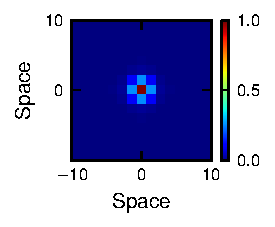
\includegraphics[scale=1]{./Figures/DisturbanceWidthEstimation0.pdf}}
\subfloat[][]{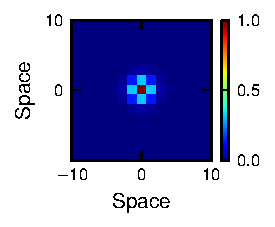
\includegraphics[scale=1]{./Figures/DisturbanceWidthEstimation01.pdf}}
\subfloat[][]{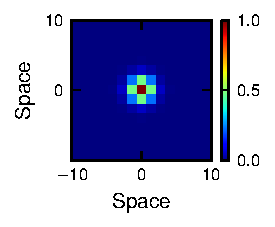
\includegraphics[scale=1]{./Figures/DisturbanceWidthEstimation02.pdf}}\\
\subfloat[][]{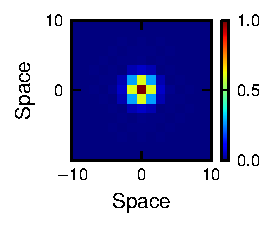
\includegraphics[scale=1]{./Figures/DisturbanceWidthEstimation023.pdf}}
\subfloat[][]{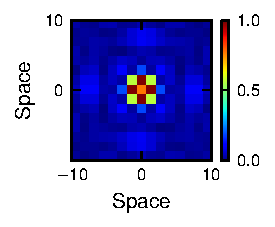
\includegraphics[scale=1]{./Figures/DisturbanceWidthEstimation03.pdf}}
\subfloat[][]{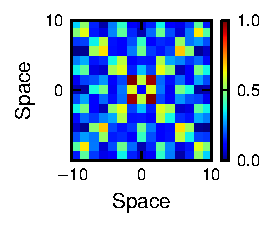
\includegraphics[scale=1]{./Figures/DisturbanceWidthEstimation04.pdf}}
\caption{{\bf Disturbance support estimates for variyng observation noise variance.} Each subplot shows the support of the disturbance covariance function convolved twice with the sensor kernel. (\textbf a) $\sigma_{\varepsilon}^2$=0. (\textbf b) $\sigma_{\varepsilon}^2$=0.1 . (\textbf c) $\sigma_{\varepsilon}^2$=0.2 .  (\textbf d) $\sigma_{\varepsilon}^2$=0.23 .  (\textbf e) $\sigma_{\varepsilon}^2$=0.3 . (\textbf f) $\sigma_{\varepsilon}^2$=0.4 .}
\label{fig:DisturbanceSupportExperiment}
\end{figure}
\begin{figure}[!ht]
\begin{center}
\subfloat[][]{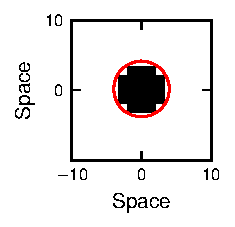
\includegraphics[scale=1]{./Figures/DisturbanceWidthEstimationBinary.pdf}}
\subfloat[][]{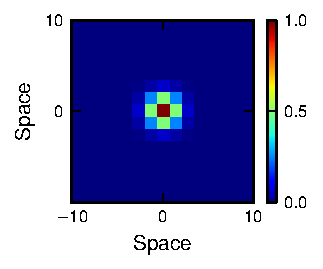
\includegraphics[scale=1]{./Figures/DisturbanceWidthTrue.pdf}}
\end{center}
\caption{{\bf Disturbance support approximation for }$\sigma_{\varepsilon}^2<$0.23. Each subplot shows the support of the disturbance covariance function convolved twice with the sensor kernel. (\textbf{a}) Estimated support is shown by red circle, nonzero values after thresholding are shown by the black area. (\textbf{b}) True support.}
\label{fig:BinaryDisturbanceWidthEstimation}
\end{figure}
\begin{figure}[!ht]
\begin{center}
\centering
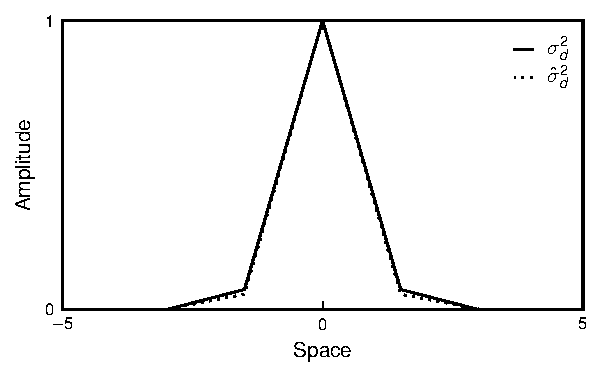
\includegraphics[scale=1]{./Figures/DisturbanceWidthEstimationCrossSection.pdf}
\end{center}
\caption{{\bf Cross-section of disturbance covariance support estimation}. The normalized true and the estimated width are shown by solid and dashed lines respectively.}
\label{fig:DisturbanceWidthEstimationCrossSection}
\end{figure}
\begin{figure}
\begin{center}
\subfloat[][]{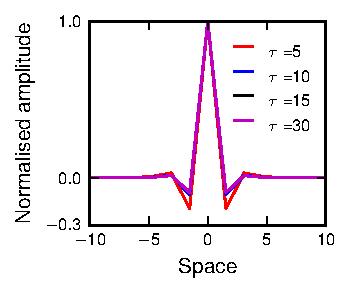
\includegraphics[scale=.8]{./Figures/KernelSupportForObservationNoise0.pdf}}
\subfloat[][]{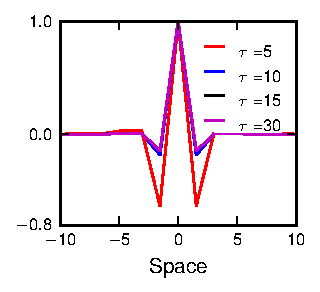
\includegraphics[scale=.8]{./Figures/KernelSupportForObservationNoise01.pdf}}
\subfloat[][]{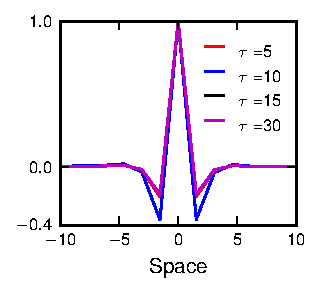
\includegraphics[scale=.8]{./Figures/KernelSupportForObservationNoise018.pdf}}
\end{center}
\caption{{\bf Kernel support approximation for different values of synaptic time constant, $\tau$ and observation noise variance, $\sigma^2_{\varepsilon}$}. Each subplot shows normalised connectivity kernel estimate. (\textbf a) $\sigma_{\varepsilon}^2$=0. (\textbf b) $\sigma_{\varepsilon}^2$=0.1 . (\textbf c) $\sigma_{\varepsilon}^2$=0.18.}
\label{fig:KernelWidthEstimationExperiment}
\end{figure}
The effect of the observation noise variance on the connectivity kernel support is very much like to that of disturbance covariance function where an initial guess can be made in a similar manner. To study how synaptic parameter, $\xi=1-\frac{ T_s}{\tau}$, influence the resultant support of the connectivity kernel different values of synaptic time constatnt, $\tau$, were considered in a physiologically plausible range while noting that its value should be also higher than the sampling time. In fact synaptic parameter in \eqref{eq:EM-Fourier_TF_of_Kernel}  acts like a scaling factor, dilating or shrinking the estimated support, as the subtracting a constant in a frequency domain only affects the value at the origin in the spatial domain. The result of the correlation analysis for the connectivity kernel is shown in Figure~\ref{fig:KernelWidthEstimationExperiment} where each subplot is the normalised  estimate for varying synaptic time constants while the observation noise was kept constant. Note that for clarification the amplitude at the origin was negated when the chosen values of $\tau$ and $\sigma^2_{\varepsilon}$ resulted in the negative values at the origin. The result suggests that choosing the range of approximately $\left[-5,5 \right] $ is reasonable for the spatial extent of the connectivity kernel.


 By doing so, the exact shape of the kernel and disturbance covariance function cannot be inferred, this step might be considered as an initialisation for the EM algorithm, however, an approximate of their support can be still extracted. In fact, the estimated support for the disturbance covariance function was very accurate. The estimates of the connectivity kernel and disturbance support were normalised and thresholded for values less than 0.01. The result of the correlation analysis for the connectivity kernel is shown in Figure.\ref{fig:KernelWidthEstimation}. The red circle shows the estimated support which encompasses the non-zero values (black area) after thresholding. The estimated support of the disturbance covariance function convolved twice with the observation kernel is shown in Figure.\ref{fig:DisturbanceWidthEstimation}. By fitting a Guassian basis function to the result, and under the assumption that the width of the sensor, $\sigma_m^2$ were known, the width of the disturbance covariance function, $\sigma_d^2$ was calculated analytically using the expression for Gaussian basis functions convolution.

The estimated supports were then employed in the EM algorithm described in Section \ref{sec:EstimationAlgorithm} to estimate the smoothed states $\hat{\mathbf x}_t^b$, the connectivity kernel weights $\boldsymbol\theta$, the synaptic dynamic $\xi$, and the hyperparameters $\sigma_{\epsilon}^2$ and $\sigma^2_d$. A  square grid of $n_{\theta}=25$ (5 by 5) basis functions with $2.25~mm$ spacing were used to cover the estimated kernel support where $\sigma_{\psi}^2=3.5$. This is shown in Figure.\ref{fig:KernelWidthEstimation} by blue circles, each of which representing full width at half maximum of the connectivity kernel basis functions. The true and estimated connectivity kernel for 100 Monte Carlo simulations are shown in Figure~\ref{fig:KernelEstimates}. Cross-sections of the connectivity kernel estimates for each run are shown in Figure~\ref{fig:KernelEstimateCrossSection}. The reconstructed kernel is in good accordance with the actual kernel, where the actual kernel is inside the confidence interval. The large standard deviation is due to the high number of parameters need to be estimated. Figure~\ref{fig:Histogram} depicts the histogram of parameter estimates from 100 simulations where the true parameter value is shown by the solid line and the mean parameter estimate is shown by the dashed line. These histograms indicate small bias in parameter estimates with a very small standard deviation. Examples of neural field reconstruction are given in Figure.~\ref{fig:FieldEstimates}.  The figure shows snapshots at three time instants of the true neural field and the estimated field. In each subplot neural activity is plotted against spatial index in 1D to provide a comparision between true and the estimated underlying fields. Plot of lower bound of the log likelihood versus iterations of the EM is shown in Figure.~\ref{fig:LowerBound}. In general, for the non-linear dynamical systems the actual lower bound can not be claculated analytically, therefore the approximate of the lower bound obtained by URTSS is shown. The change in lower bound drops below 0.009 percent after 15 iterations, confirming
that the algorithm converged to steady parameter values.
\section{Discussion}
The correlation analysis specifies approximate supports for both disturbance covariance function and connectivity kernel. Although the unknown parameters $\xi$ and $\sigma_{\varepsilon}^2$ can be set as described in \S~\ref{subsec:CorrAnal}, the chosen values influence the exact shape of the kernel significantly, the analysis also assumes the sigmoidal firing rate to be in the active region, as a result  the kernel and the disturbance amplitudes cannot be inferred only through correlation analysis. This step might be considered as a prerequisite for the EM algorithm described in \S~\ref{sec:EstimationAlgorithm} where approximated supports are employed to estimate the gain of the kernel and disturbance. Knowing the spatial extent of the kernel greatly increases the speed of the algorithm as the number of basis functions to decompose the kernel reduces significanly compared to the case in which the basis funtions are laid out across the entire spatial domain. This also improves the uncertainty of the estimates because of the lower number of parameters needs to be estimated. On the other hand, the approximated support of the disturbance covariance function facilitates the implementation of the EM algorithm as the disturbance covariance matrix can be factorised into two components, a constant matrix depending only on the inferred support and an unknown scaling parameter. This way the problem of estimating the covariance matrix reduces to estimation of a single scaling parameter.

The additional Taylor expansion step inroduced in the E-step resembles the extended Kalman filtering (EKF) \cite{Jazwinski1970,Chui2009} in which a stationary nonlinear dynamic system is approximated by a linear non-stationary system using the first order Taylor approximation of the nonlinear equations about the state estimates. This may suggest that the extended Kalman smoother is a natural approach to infer the sequence of state vecors in the presented framework. However, extended Kalman smoother (EKS) requires relinearising about the backwards estimates which in turn necessitates the nonlinear mapping to be uniquely invertible. Although this is indeed the case in the neural field equation employed in this work it will impose more computational complexity in the state estimation procedure. In addition, URTSS provides better state approximation compared to the EKS \cite{Haykin2001} and therefore the approximated lower bound will be more accurate  resulting in better parameter estimations.

While EKS has been  applied in the context of EM algorithm for learning a nonlinear model from data \cite{Ghahramani1999} this is the first work (to the best authors' knowlege) where the URTSS has been used to perform state inference in the E-step of the EM algorithm. However, as in the case of EKS since an approximate lower bound is maximised at each time step there is no guarantee that URTSS increases the lower bound on the true likelihood function and therefore the stability of the algorithm cannot be ensured. Nevertheless, the proposed framework is more stable due to better performance of the URTSS.

In almost all applications a sequence of likelihood converges to some stationary values i.e. global (local) maximum or a saddle point. If the sequence of EM is trapped in a saddle point a small random purturbation diverges the EM from the saddle point \cite{McLachlan1997}. In general convergence of the EM algorithm to any stationary point either global (local) maxima or saddle points 
depends on the initialisation. Here a bounded sequence of state vectors were used to initialise the algorithm which gives a satisfactory convergence and good state and good parameter estimations.

Since the non-linearity is a sigmoid function first-order Taylor approximation provides a good approximation to the lower bound of the likelihood function, however in general settings with more complicated nonlinear behaviours higher order terms might need to be included, this however introduces intractable computational complexity.
\begin{itemize}
	\item itterative EM and correlation analysis (maybe)
\end{itemize}
\scetion{Conclusion}

% % all figures here
% % ~~~~~~~~~~~~~~~~

\begin{figure}[!ht]
\begin{center}
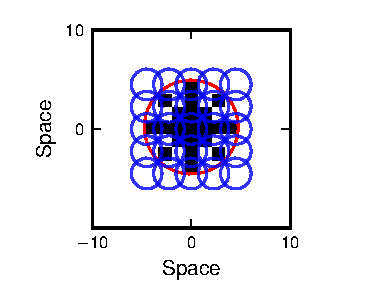
\includegraphics{./Figures/KernelBasis1.pdf}
\end{center}
\caption{{\bf Connectivity kernel support approximation.} The approximate support of the kernel is shown by the red circle. Black area shows the non-zero values of the support after thresholding. A $5\times5$ grid of basis functions (blue circles) used to reconstruct the connectivity kernel.}
\label{fig:KernelWidthEstimation}
\end{figure}
%~~~~~~~~~~~~~~~~~~~~~~~~~~~~~~~~~
\begin{figure}[!ht]
\begin{center}
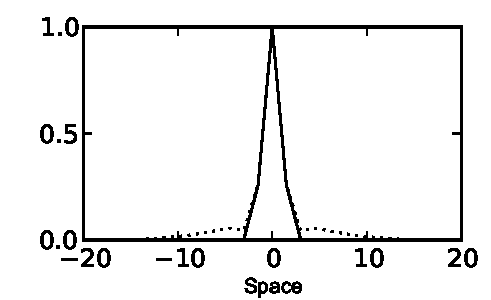
\includegraphics{./Figures/DisturbanceWidthEstimation.pdf}
\end{center}
\caption{{\bf Disturbance support approximation}. }
\label{fig:DisturbanceWidthEstimation}
\end{figure}
%~~~~~~~~~~~~~~~~~~~~~~~~~~~~~~~~~~~~~
\begin{figure}[!ht]
\begin{center}
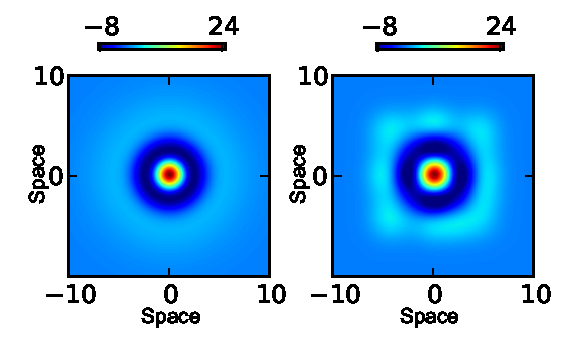
\includegraphics{./Figures/KernelEstimate.pdf}
\end{center}
\caption{{\bf Connectivity kernel estimates.} (A) Actual kernel. (B) The mean kernel estimate over 100 realisations.}
\label{fig:KernelEstimates}
\end{figure}
%~~~~~~~~~~~~~~~~~~~~~~~~~~~~~~~~~~~~~
\begin{figure}[!ht]
\begin{center}
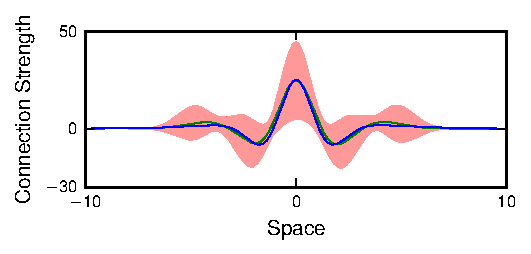
\includegraphics{./Figures/KernelEstimateCrossSection.pdf}
\end{center}
\caption{{\bf Cross-sections of connectivity kernel estimates.} Actual kernel and the mean kernel estimates are shown with blue and green lines respectively. Each of the estimate from Monte Carlo simulation is shown with black line. The 95\% confidence intervals are shown by shaded red area.}
\label{fig:KernelEstimateCrossSection}
\end{figure}
%~~~~~~~~~~~~~~~~~~~~~~~~~~~~~~~~~~~~~~
\begin{figure}[!ht]
\begin{center}
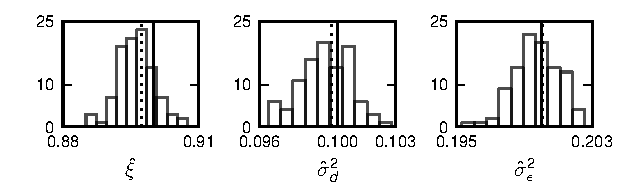
\includegraphics{./Figures/Histogram.pdf}
\end{center}
\caption{{\bf Histograms of the parameter estimates over 100 realizations}. The actual and mean of the estimated parameter values are shown by solid and dotted lines respectively. (A) The histogram of the synaptic dynamic parameter, $\xi$. (B) The histogram of the observation noise variance, $\sigma_{\epsilon}$. (C) The histogram of the disturbance noise variance, $\sigma_d^2$.}
\label{fig:Histogram}
\end{figure}
%~~~~~~~~~~~~~~~~~~~~~~~~~~~~~~~~~~~~~~~~
\begin{figure}[!ht]
\begin{center}
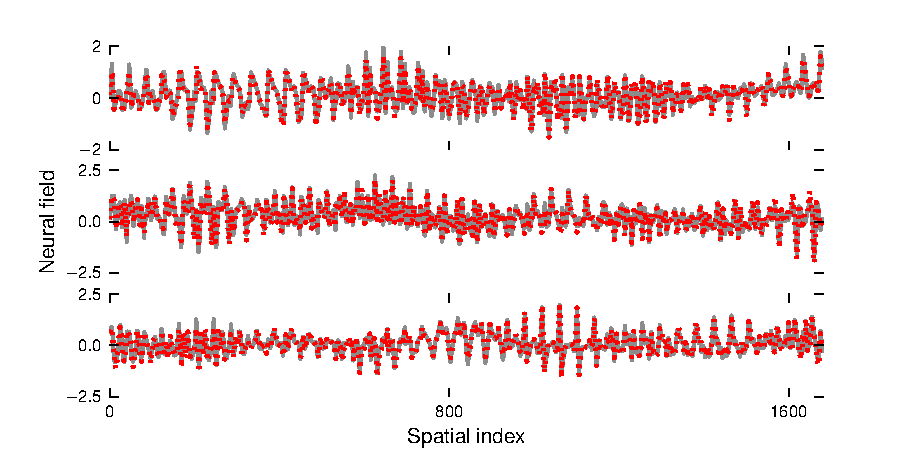
\includegraphics[scale=1]{./Figures/FieldEstimates.pdf}
\end{center}
\caption{{\bf Neural field estimates at different time instants}. In each subplot, true (gray line) and reconstructed neural field (red dots) are plotted versus spatial index.}
\label{fig:FieldEstimates}
\end{figure}
%~~~~~~~~~~~~~~~~~~~~~~~~~~~~~~~~~~~~~~~~~
\begin{figure}[!ht]
\begin{center}
\includegraphics{./Figures/Q.pdf}
\end{center}
\caption{{\bf Convergence of the EM algorithm.} The mean of the lower bound of the log-likelihood function over 100 realisations. The change in lower bound drops below 0.009 percent after 15 iterations}
%  $Q(\boldsymbol\Theta',\boldsymbol\Theta')=-(T-1)\left[n_y(1+\ln \hat{\sigma}^2_{\epsilon})+ n_x(1+\ln \hat{\sigma}^2_d)\right]$
\label{fig:LowerBound}
\end{figure}
%~~~~~~~~~~~~~~~~~~~~~~~~~~~~~~~~~~~~~~~~
\begin{figure}[!ht]
\centering
% \subfloat[][]{\includegraphics[scale=1]{./Graph/EM/Q.pdf}}\\
\subfloat[][]{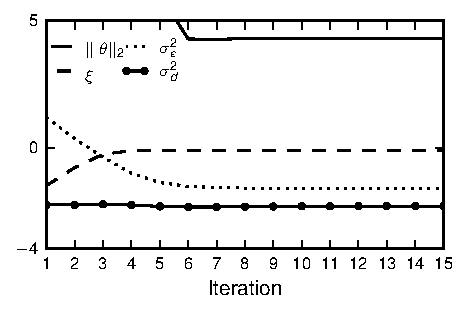
\includegraphics[scale=1]{./Figures/ParameterConvergence.pdf}}\\
\centering
\subfloat[][]{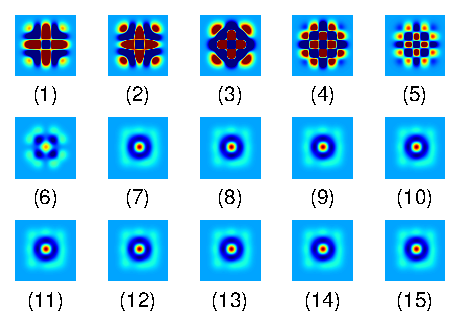
\includegraphics[scale=1]{./Figures/KernelConvergence.pdf}}
\caption{{\bf Convergence of parameters}. All parameters converge after 9 iterations. (\textbf a) The logarithm of the mean of synaptic parameter, observation noise variance and field disturbance variance over 100 realisations. (\textbf b) The mean kernel estimates at each iteration of the EM algorithm.}
\label{fig:ParameterConvergence}
\end{figure}

\clearpage
\newpage
\appendix
\section{Product of two $n$-dimensional Gaussian functions}\label{sec:GaussianProduct} 
In this section, we provide a derivation for the product of two n-dimensional Gaussian basis functions.
This derivation is used in the  calculation of $\boldsymbol\Lambda_t^{(i)}$  defined in equation \eqref{eq:EM-Lambdat} of the main text. Consider two
Gaussian basis functions
\begin{equation}\label{eq:n_dimensional_Gaussian1}
 \varphi_i(\mathbf r)=\mathrm{exp}\left({-\frac{1}{\sigma_i^2} (\mathbf r-\boldsymbol \mu_i)^\top(\mathbf r-\boldsymbol \mu_i})\right)
\end{equation}
and 
\begin{equation}\label{eq:n_dimensional_Gaussian2}
\varphi_j(\mathbf r)=\mathrm{exp}\left({-\frac{1}{\sigma_j^2} (\mathbf r-\boldsymbol \mu_j)^\top(\mathbf r-\boldsymbol \mu_j})\right).
\end{equation}
the product of two Gauusian basis functions is given by
\begin{equation}
 \varphi_i(\mathbf r)\varphi_j(\mathbf r)=\mathrm{exp}\left(-\left[ {\frac{1}{\sigma_i^2} (\mathbf r-\boldsymbol \mu_i)^\top(\mathbf r-\boldsymbol\mu_i)+{\frac{1}{\sigma_j^2} (\mathbf r-\boldsymbol \mu_j)^\top(\mathbf r-\boldsymbol\mu_j)}}\right] \right)
\end{equation}
the product is expanded to give
\begin{align} 
 \varphi_i(\mathbf r)\varphi_j(\mathbf r)&=
\mathrm{exp}\left(-\left[ \frac{(\sigma_i^2+\sigma_j^2)\left[\mathbf r^\top\mathbf r-2\mathbf r^\top \frac{\sigma_j^2\boldsymbol\mu_i+\sigma_i^2\boldsymbol\mu_j}{\sigma_i^2+\sigma_j^2}+\frac{(\sigma_j^2\boldsymbol\mu_i+\sigma_i^2\boldsymbol\mu_j)^\top(\sigma_j^2\boldsymbol\mu_i+\sigma_i^2\boldsymbol\mu_j)}{(\sigma_i^2+\sigma_j^2)^2}\right]}{\sigma_i^2\sigma_j^2}\right.\right. \nonumber\\
&\left.\left. \frac{+\frac{\sigma_i^2\sigma_j^2}{\sigma_i^2+\sigma_j^2}(\boldsymbol \mu_i-\boldsymbol\mu_j)^\top(\boldsymbol \mu_i-\boldsymbol\mu_j)}{}\right]\right) \nonumber\\
  &=\mathrm{exp}\left(-\frac{(\sigma_i^2+\sigma_j^2)\left[(\mathbf r-\frac{\sigma_j^2\boldsymbol\mu_i+\sigma_i^2\boldsymbol\mu_j}{\sigma_i^2+\sigma_j^2})^\top(\mathbf r-\frac{\sigma_j^2\boldsymbol\mu_i+\sigma_i^2\boldsymbol\mu_j}{\sigma_i^2+\sigma_j^2})\right]  }{\sigma_i^2\sigma_j^2}\right) \nonumber \\
   &\times\mathrm{exp}\left(-\frac{(\boldsymbol \mu_i-\boldsymbol\mu_j)^\top(\boldsymbol \mu_i-\boldsymbol\mu_j)}{\sigma_i^2+\sigma_j^2}\right),
\end{align}
therefore we have
\begin{equation}
 \varphi_i(\mathbf r)\varphi_j(\mathbf r)=c_{i,j}\times\mathrm{exp}\left({-\frac{1}{\sigma^2} (\mathbf r-\boldsymbol \mu)^\top(\mathbf r-\boldsymbol\mu)}\right)
\end{equation}
where
\begin{equation}
 c_{i,j}=\mathrm{exp}\left(-\frac{(\boldsymbol \mu_i-\boldsymbol\mu_j)^\top(\boldsymbol \mu_i-\boldsymbol\mu_j)}{\sigma_i^2+\sigma_j^2}\right) \quad \sigma^2=\frac{\sigma_i^2\sigma_j^2}{\sigma_i^2+\sigma_j^2}
\end{equation}
and
\begin{equation}
 \boldsymbol\mu=\frac{\sigma_j^2\boldsymbol\mu_i+\sigma_i^2\boldsymbol\mu_j}{\sigma_i^2+\sigma_j^2}
\end{equation}

\section{Cross-correlation and convolution}\label{ap:CorrelationAnalysis}
This appendix provide a proof for the properties of the cross-correlation and convolution used in the Correlation analysis Section of Chapter 2. To show 
\begin{equation}\label{eq:app-ConvXcorRelation1}
 \left(a \ast b \right)\left(\boldsymbol\iota\right)  \star c\left(\boldsymbol\iota\right)  = a\left(-\boldsymbol\iota\right)\ast\left(b \star c\right)\left(\boldsymbol\iota\right)
\end{equation}
and
\begin{equation}\label{eq:app-ConvXcorRelation2}
(a \ast b)(\boldsymbol \iota) \star (a \ast b)(\boldsymbol\iota)=(a \star a)(\boldsymbol\iota)\ast(b \star b)(\boldsymbol\iota),
\end{equation}
first note that cross-correlation function is related to the convolution by \cite{Yarlagadda2009}
\begin{equation}\label{eq:app-ConvXcorRelation}
 \left(a \star b\right)\left(\boldsymbol\iota\right)= a\left(-\boldsymbol\iota\right)\ast b\left(\boldsymbol\iota\right).
\end{equation}
Therefore, equation \eqref{eq:app-ConvXcorRelation1} can be wriiten as
\begin{align}
 \left(a \ast b\right)\left(\boldsymbol\iota\right) \star c\left(\boldsymbol\iota\right)&= \left(a \ast b\right)\left(-\boldsymbol\iota \right)\ast c\left(\boldsymbol\iota\right) \nonumber \\
&=a\left(-\boldsymbol\iota\right)\ast \left(b\left(-\boldsymbol\iota\right) \ast c\left(\boldsymbol\iota\right)\right)\nonumber \\
&=a\left(-\boldsymbol\iota\right)\ast\left(b\star c\right)\left(\boldsymbol\iota\right).
\end{align}
Similarly, equation \eqref{eq:app-ConvXcorRelation2} can be written as
\begin{align}
 (a \ast b)(\boldsymbol \iota) \star (a \ast b)(\boldsymbol\iota)&=(a \ast b)(-\boldsymbol\iota) \ast (a \ast b)(\boldsymbol\iota) \nonumber \\
&=a(-\boldsymbol\iota)\ast a(\boldsymbol\iota) \ast b(-\boldsymbol\iota)\ast b(\boldsymbol\iota) \nonumber \\
&=(a \star a)(\boldsymbol\iota)\ast(b \star b)(\boldsymbol\iota).
\end{align}




% \begin{figure}[!ht]
% \begin{center}
% 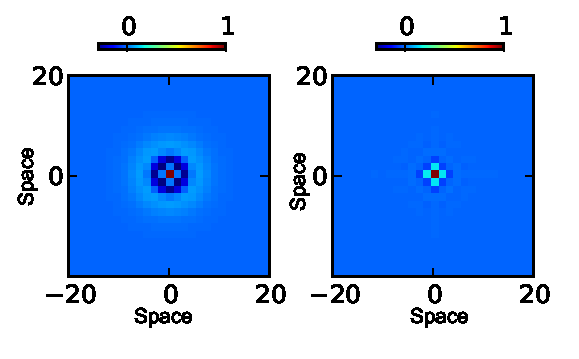
\includegraphics{./Figures/KernelWidthEstimation.pdf}
% \end{center}
% \caption{{\bf Connectivity kernel support estimation}.}
% \label{fig:KernelWidthEstimation1}
% \end{figure}
% 
% \begin{figure}[!ht]
% \begin{center}
% 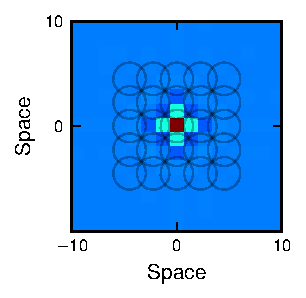
\includegraphics{./Figures/KernelBasis.pdf}
% \end{center}
% \caption{{\bf Connectivity kernel basis functions, $n_{\theta}=25$}, $\sigma^2_{\theta}=3.5$.}
% \label{fig:KernelBasis}
% \end{figure}







% \begin{figure}[!ht]
% \begin{center}
% 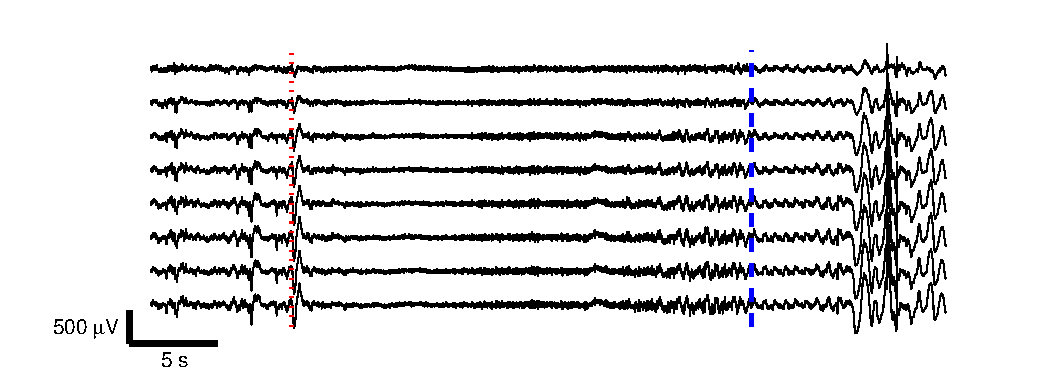
\includegraphics{./Figures/LFPs.eps}
% \end{center}
% \caption{{\bf Local field potentials from the micro-electrode array}. Data recorded from the first 8 channels of the array. The red dotted line indicates the seizure onset and the blue dashed line indicates the seizure end.}
% \label{fig:TimeSeries}
% \end{figure}
% 
% 
% \begin{figure}[!ht]
% \begin{center}
% 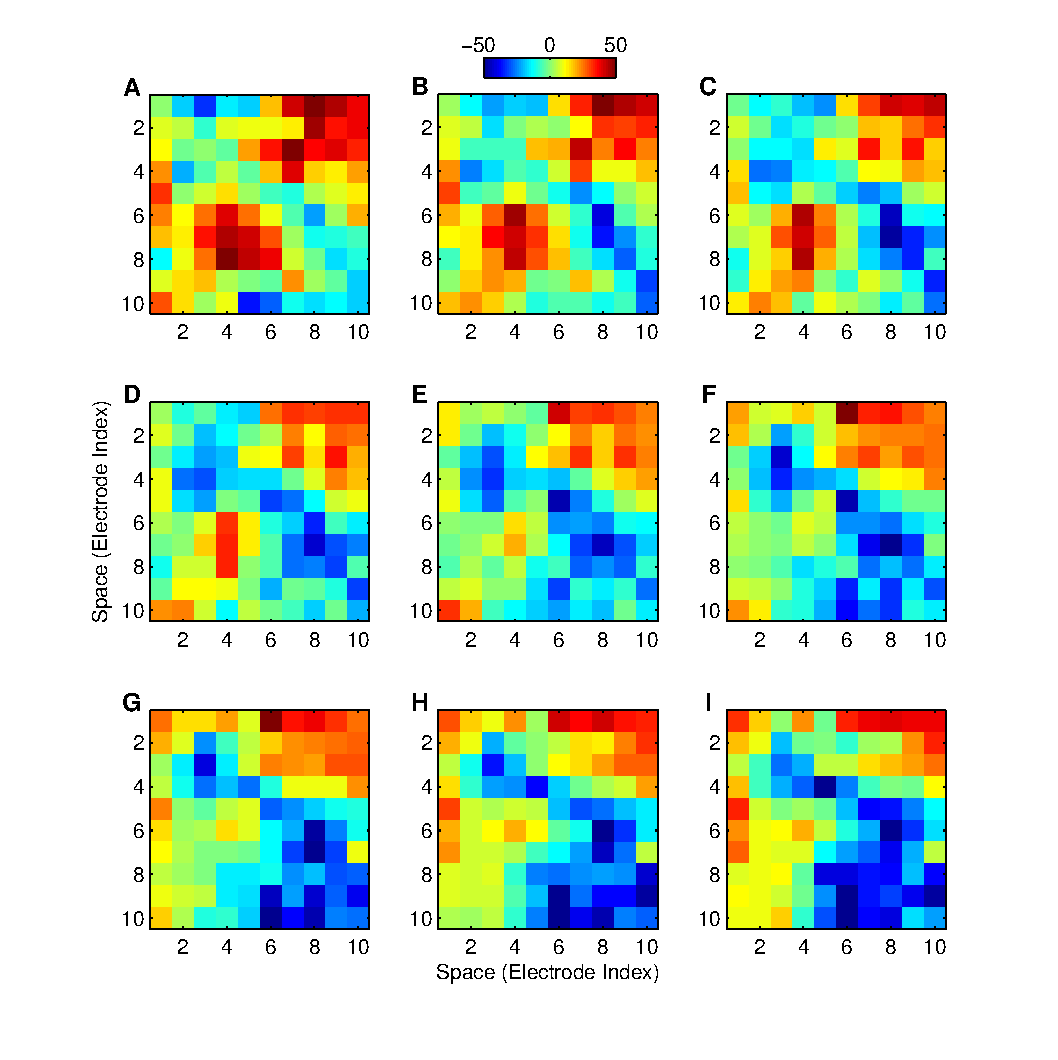
\includegraphics{./Figures/FieldObservations.eps}
% \end{center}
% \caption{{\bf Snap-shots of the spatial aspects of the observed field}. The snap-shots are ordered from A to I forming a consecutive sequence spaced 2.5~ms apart starting at 34.024s}
% \label{fig:FieldObserations}
% \end{figure}
% 
% \begin{figure}[!ht]
% \begin{center}
% 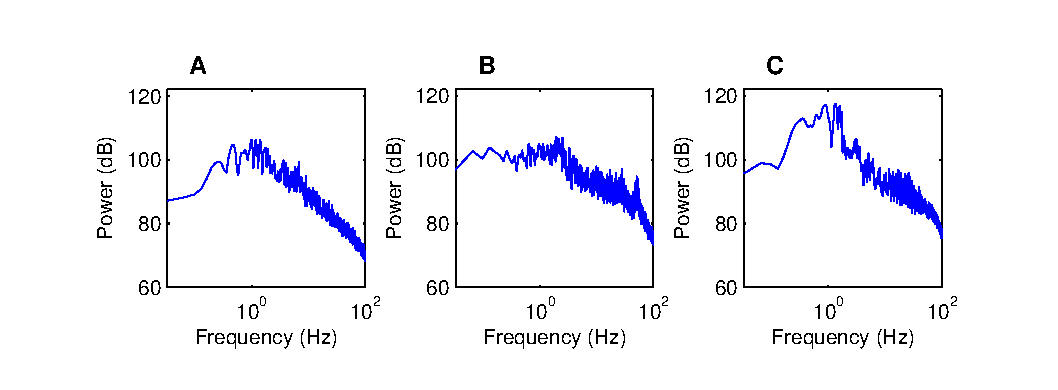
\includegraphics{./Figures/TemporalFreq.eps}
% \end{center}
% \caption{{\bf Spectra from local field potential recordings}. A. Pre-seizure observations. B. Seizure observations. C. Post-seizure observations.}
% \label{fig:TemporalFreqObservation}
% \end{figure}
% 
% \begin{figure}[!ht]
% \begin{center}
% 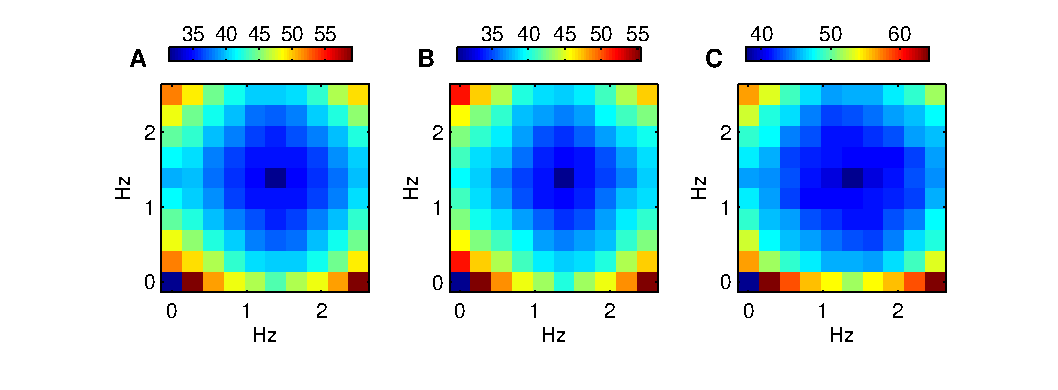
\includegraphics{./Figures/SpatialFreq.eps}
% \end{center}
% \caption{{\bf Spatial frequency analysis of the observed neural field}. A. Pre-seizure observations. B. Seizure observations. C. Post-seizure observations.}
% \label{fig:SpatialFreqObservation}
% \end{figure}
% 
% \begin{figure}[!ht]
% \begin{center}
% 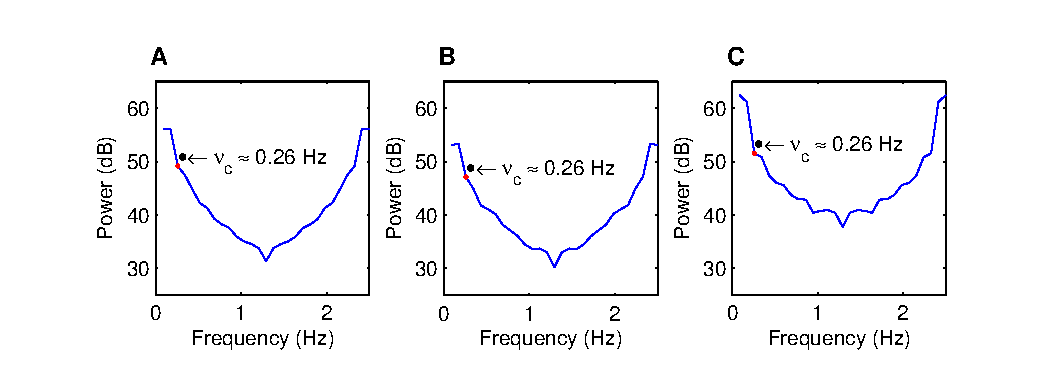
\includegraphics{./Figures/SpatialFreqCrossSection.eps}
% \end{center}
% \caption{{\bf Diagonal cross-section of the spatial frequency plots of the observed neural field}. A. Pre-seizure observations. B. Seizure observations. C. Post-seizure observations.}
% \label{fig:DiagSpatialFreqObservation}
% \end{figure}
% 
% \begin{figure}[!ht]
% \begin{center}
% 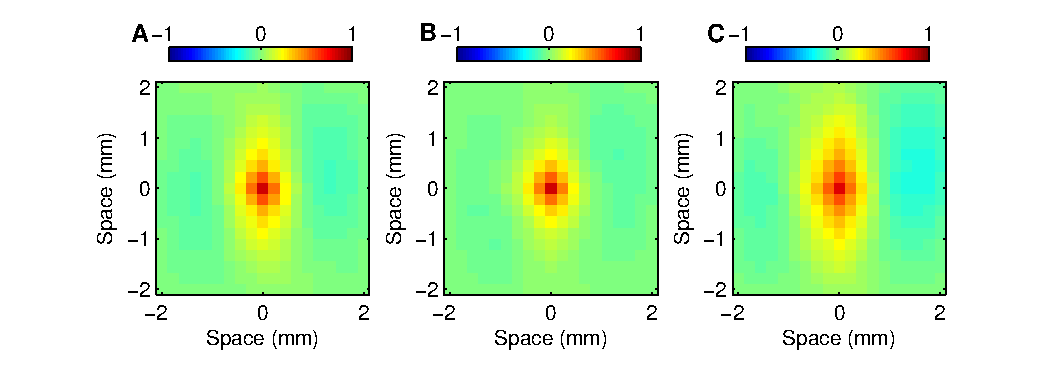
\includegraphics{./Figures/CrossCorr2D.eps}
% \end{center}
% \caption{{\bf Mean cross-correlations between consecutive observations of the neural field}. Note: The correlations are normalised such that the maximum value is one. A. Pre-seizure observation correlations. B. Seizure observation correlations. C. Post-seizure observation correlations.}
% \label{fig:SpatialCrossCorrelation}
% \end{figure}
% 
% \begin{figure}[!ht]
% \begin{center}
% 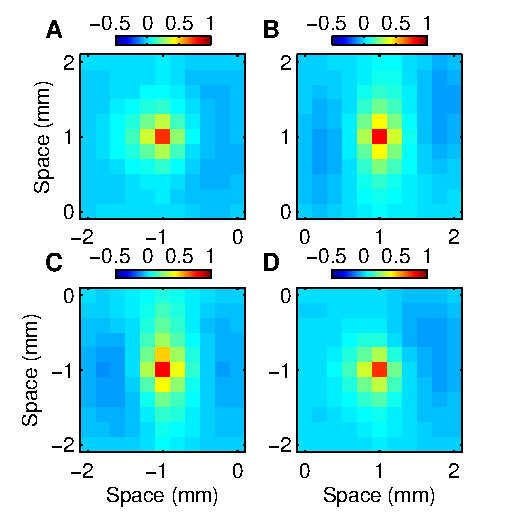
\includegraphics{./Figures/HomoTestCrossCorr.eps}
% \end{center}
% \caption{{\bf Mean cross-correlations between consecutive samples using subsets of observations of the neural field}. Each subplot shows correlations corresponding to a subset electrodes. Indexing the electrodes in a (x,y) grid, where index ranges from 1 to 10. Subplot A shows the mean correlation between electrode indexes (1-6, 5-10), subplot B shows correlations from indexes (5-10,5-10), subplot C shows indexes (1-6, 1-6) and subplot D shows indexes (5-10, 5-10).}
% \label{fig:HomogeneityTest}
% \end{figure}

% tables here
% ~~~~~~~~~~~
\renewcommand{\arraystretch}{1.7}
\begin{table}[!ht]
\caption{
\bf{Algorithm for the Unscented RTS Smoother}}
\label{tab:URTSSAlgorithm}
\begin{tabular}{|c|}\hline
\multicolumn{1}{|p{16cm}|}{\textbf{1.} Forward initialisation} \\ 
$\hat{\mathbf x}_0, \mathbf P_0$ \\
\hline
\multicolumn{1}{|p{16cm}|}{\textbf{2.} Forward iteration: for $t \in \left\lbrace 0,\cdots, T\right\rbrace $, calculate the sigma points $\mathcal X_{i,t}^f$ using equations \ref{eq:sigmapoints1}-\ref{eq:sigmapoints3} and propagate through equation~\ref{eq:QmatrixForSigmapoints}} \\
$\mathcal X_{i,t+1}^{f-}=Q(\mathcal X_{i,t}^f) \quad i=0, \dots, 2L$\\
\multicolumn{1}{|p{16cm}|}{Calculate the predicted state and the predicted covariance matrix} \\
$\hat{\mathbf x}_{t+1}^{f-}=\sum_{i=0}^{2L} W_i^{(m)}\mathcal X_{i,t+1}^{f-} $ \\
$\mathbf P_{t +1}^{f-}=\sum_{i=0}^{2L} W_i^{(c)}(\mathcal X_{i,t+1}^{f-}-\hat{\mathbf x}_{t +1}^{f-})(\mathcal X_{i,t+1}^{f-}-\hat{\mathbf x}_{t +1}^{f-})^\top+\boldsymbol \Sigma_e$ \\ 
\multicolumn{1}{|p{16cm}|}{Compute the filter gain, the filtered state and the filtered covariance matrix using the standard Kalman filter update equations} \\
$\mathcal K_{t+1}=\mathbf P_{t +1}^{f-}\mathbf C ^\top(\mathbf C \mathbf P_{t +1}^{f-}\mathbf C ^\top+\boldsymbol \Sigma_{\varepsilon})^{-1}$\\
$\hat{\mathbf x}_{t+1}^{f}=\hat{\mathbf x}_{t+1}^{f-}+\mathcal K_{t+1}(\mathbf y_{t+1}-\mathbf C\hat{\mathbf x}_{t +1}^{f-}) $\\
$\mathbf P_{t+1}^f=(\mathbf I - \mathcal K_{t+1}\mathbf C)\mathbf P_{t +1}^{f-}$\\ 
\hline
\multicolumn{1}{|p{16cm}|}{\textbf{3.} Backward initialisation}\\
$\mathbf P_T^b= \mathbf P_T^f, \quad \hat{\mathbf x}^b_T= \hat{\mathbf x}^f_T$ \\
\hline
\multicolumn{1}{|p{16cm}|}{\textbf{4.} Backward iteration: for $t \in \left\lbrace T-1, \cdots, 0 \right\rbrace $ calculate the sigma points $\mathcal X_{i,t}^b$ and propagate them through equation \ref{eq:QmatrixForSigmapoints}}\\
$\mathcal X_{i,t+1}^{b-}=Q(\mathcal X_{i,t}^b) \quad i=0, \dots, 2L$\\
\multicolumn{1}{|p{16cm}|}{Calculate the predicted state and the predicted covariance matrix}\\
$\hat{\mathbf x}_{t+1}^{b-}=\sum_{i=0}^{2L} W_i^{(m)}\mathcal X_{i,t+1}^{b-}$\\
$\mathbf P_{t +1}^{b-}=\sum_{i=0}^{2L} W_i^{(c)}(\mathcal X_{i,t+1}^{b-}-\hat{\mathbf x}_{t +1}^{b-})(\mathcal X_{i,t+1}^{b-}-\hat{\mathbf x}_{t +1}^{b-})^\top+\boldsymbol \Sigma_e $\\
$\mathbf M_{t +1}^{b-}=\sum_{i=0}^{2L} W_i^{(c)}(\mathcal X_{i,t}^{b-}-\hat{\mathbf x}_{t}^{f})(\mathcal X_{i,t+1}^{b-}-\hat{\mathbf x}_{t+1}^{b-})^\top$\\
\multicolumn{1}{|p{16cm}|}{Compute the smoother gain, the smoothed state and the smoothed covariance matrix}\\
$\mathbf S_t=\mathbf M_{t +1}^{b-}\left[ \mathbf P_{t +1}^{b-}\right] ^{-1} $\\
$\hat{\mathbf x}_t^b=\hat{\mathbf x}_t^f+\mathbf S_t\left[\hat{\mathbf x}_{t+1}^{b}-\hat{\mathbf x}_{t+1}^{b-}\right]$\\
$\mathbf P_{t}^{b}=\mathbf P_{t}^{f}+\mathbf S_t\left[\mathbf P_{t+1}^{b}-\mathbf P_{t+1}^{b-} \right]\mathbf S_t^\top $\\
\multicolumn{1}{|p{16cm}|}{Additional step to calculate the smoothed cross covariance matrix \cite{Sarkka2008}} \\
$\mathbf M_{t +1}^{b}=\mathbf S_t\mathbf P_{t+1}^{b}$\\
\hline
\end{tabular}
\begin{flushleft}This table shows the steps in the unscented Rauch-Tung-Striebel smoother algorithm. The steps are iterated 11 times for our state estimation procedure. The least squares algorithm is run after each iteration to update the parameter estimates.
\end{flushleft}
\label{tab:UKFAlgorithm}
\end{table}
 \renewcommand{\arraystretch}{1}
\clearpage
\newpage
\bibliographystyle{plain}
\bibliography{EMIDE}
\end{document}
